\chapter{Proposed Framework}
\label{chap:framework}
In this chapter, we will introduce our proposed framework(see Figure~\ref{fig:my_model}) based on the Transformer models in detailed.But before that, we would like to explain our thoughts on the preliminary stage of the thesis, our first method: Pixel-base attention.


\section{Pixel-based attention}\label{sec:pixel_base}

We are inspired by Encoder Self-Attention in DETR, and its output attention map can intuitively distinguish each object in the image(see Figure~\ref{fig:detrattentionmap}). Therefore, we envisage using multi-self attention to intuitively distinguish the relationship between objects in the image.

\subsection{Idea of Pixel-based attention}

We input the down-sampled image features into the Multihead Self-Attention module. According to the Equation~\ref{equ:self_attention}, we will get the attention weight between each pixel in the down-sampled image feature. Assuming that in Figure~\ref{fig:ideamethod1} we obtained the down-sampled image feature size of 512x66x50 through the backbone, that is, each layer od the feature has 3300 pixels, we convert it into a sequence of 3300x512, then input it into the Multihead Self-Attention module, and get an attention map size of 3300x3300 . We look for the pixel of the subject in the row of the attention map, and look for the pixel of the object in the column of the attention map ,to find the attention weight between the subject and object pixels. Eg. the ground truth pair $ \left\langle roof, building \right \rangle $ in Figure~\ref{fig:ideamethod1} is located in the attention map as shown in the lower right corner of Figure ~\ref{fig:ideamethod1}.

We hope that through the training of our model, the attention weight of ground truth pairs can be higher than those of pairs without relation. In this way, we can use the attention weight in the evaluation to determine which pairs are most likely to be related.
\begin{figure}[!htbp]
		\centering
	\subfigure[No relation between \textit{roof} and \textit{tree}.]{
		\begin{minipage}[t]{6cm}
			\centering
			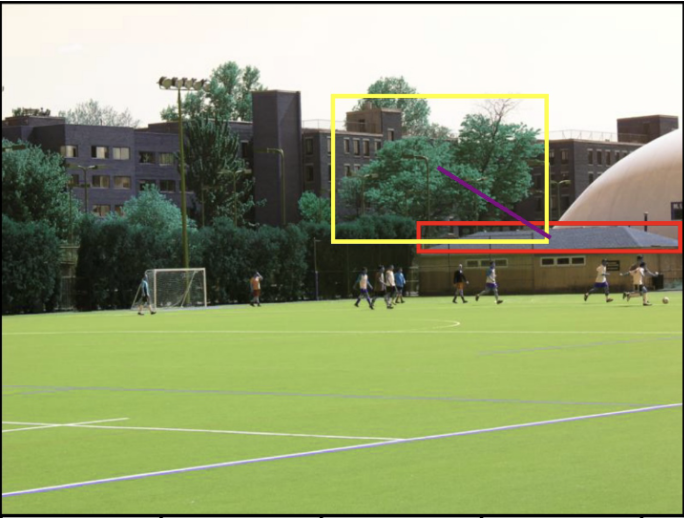
\includegraphics[width=1\linewidth]{figures/roof/img1}
	\end{minipage}}
	\subfigure[The attention of $<roof, tree>$.]{
		\begin{minipage}[t]{6cm}
			\centering
			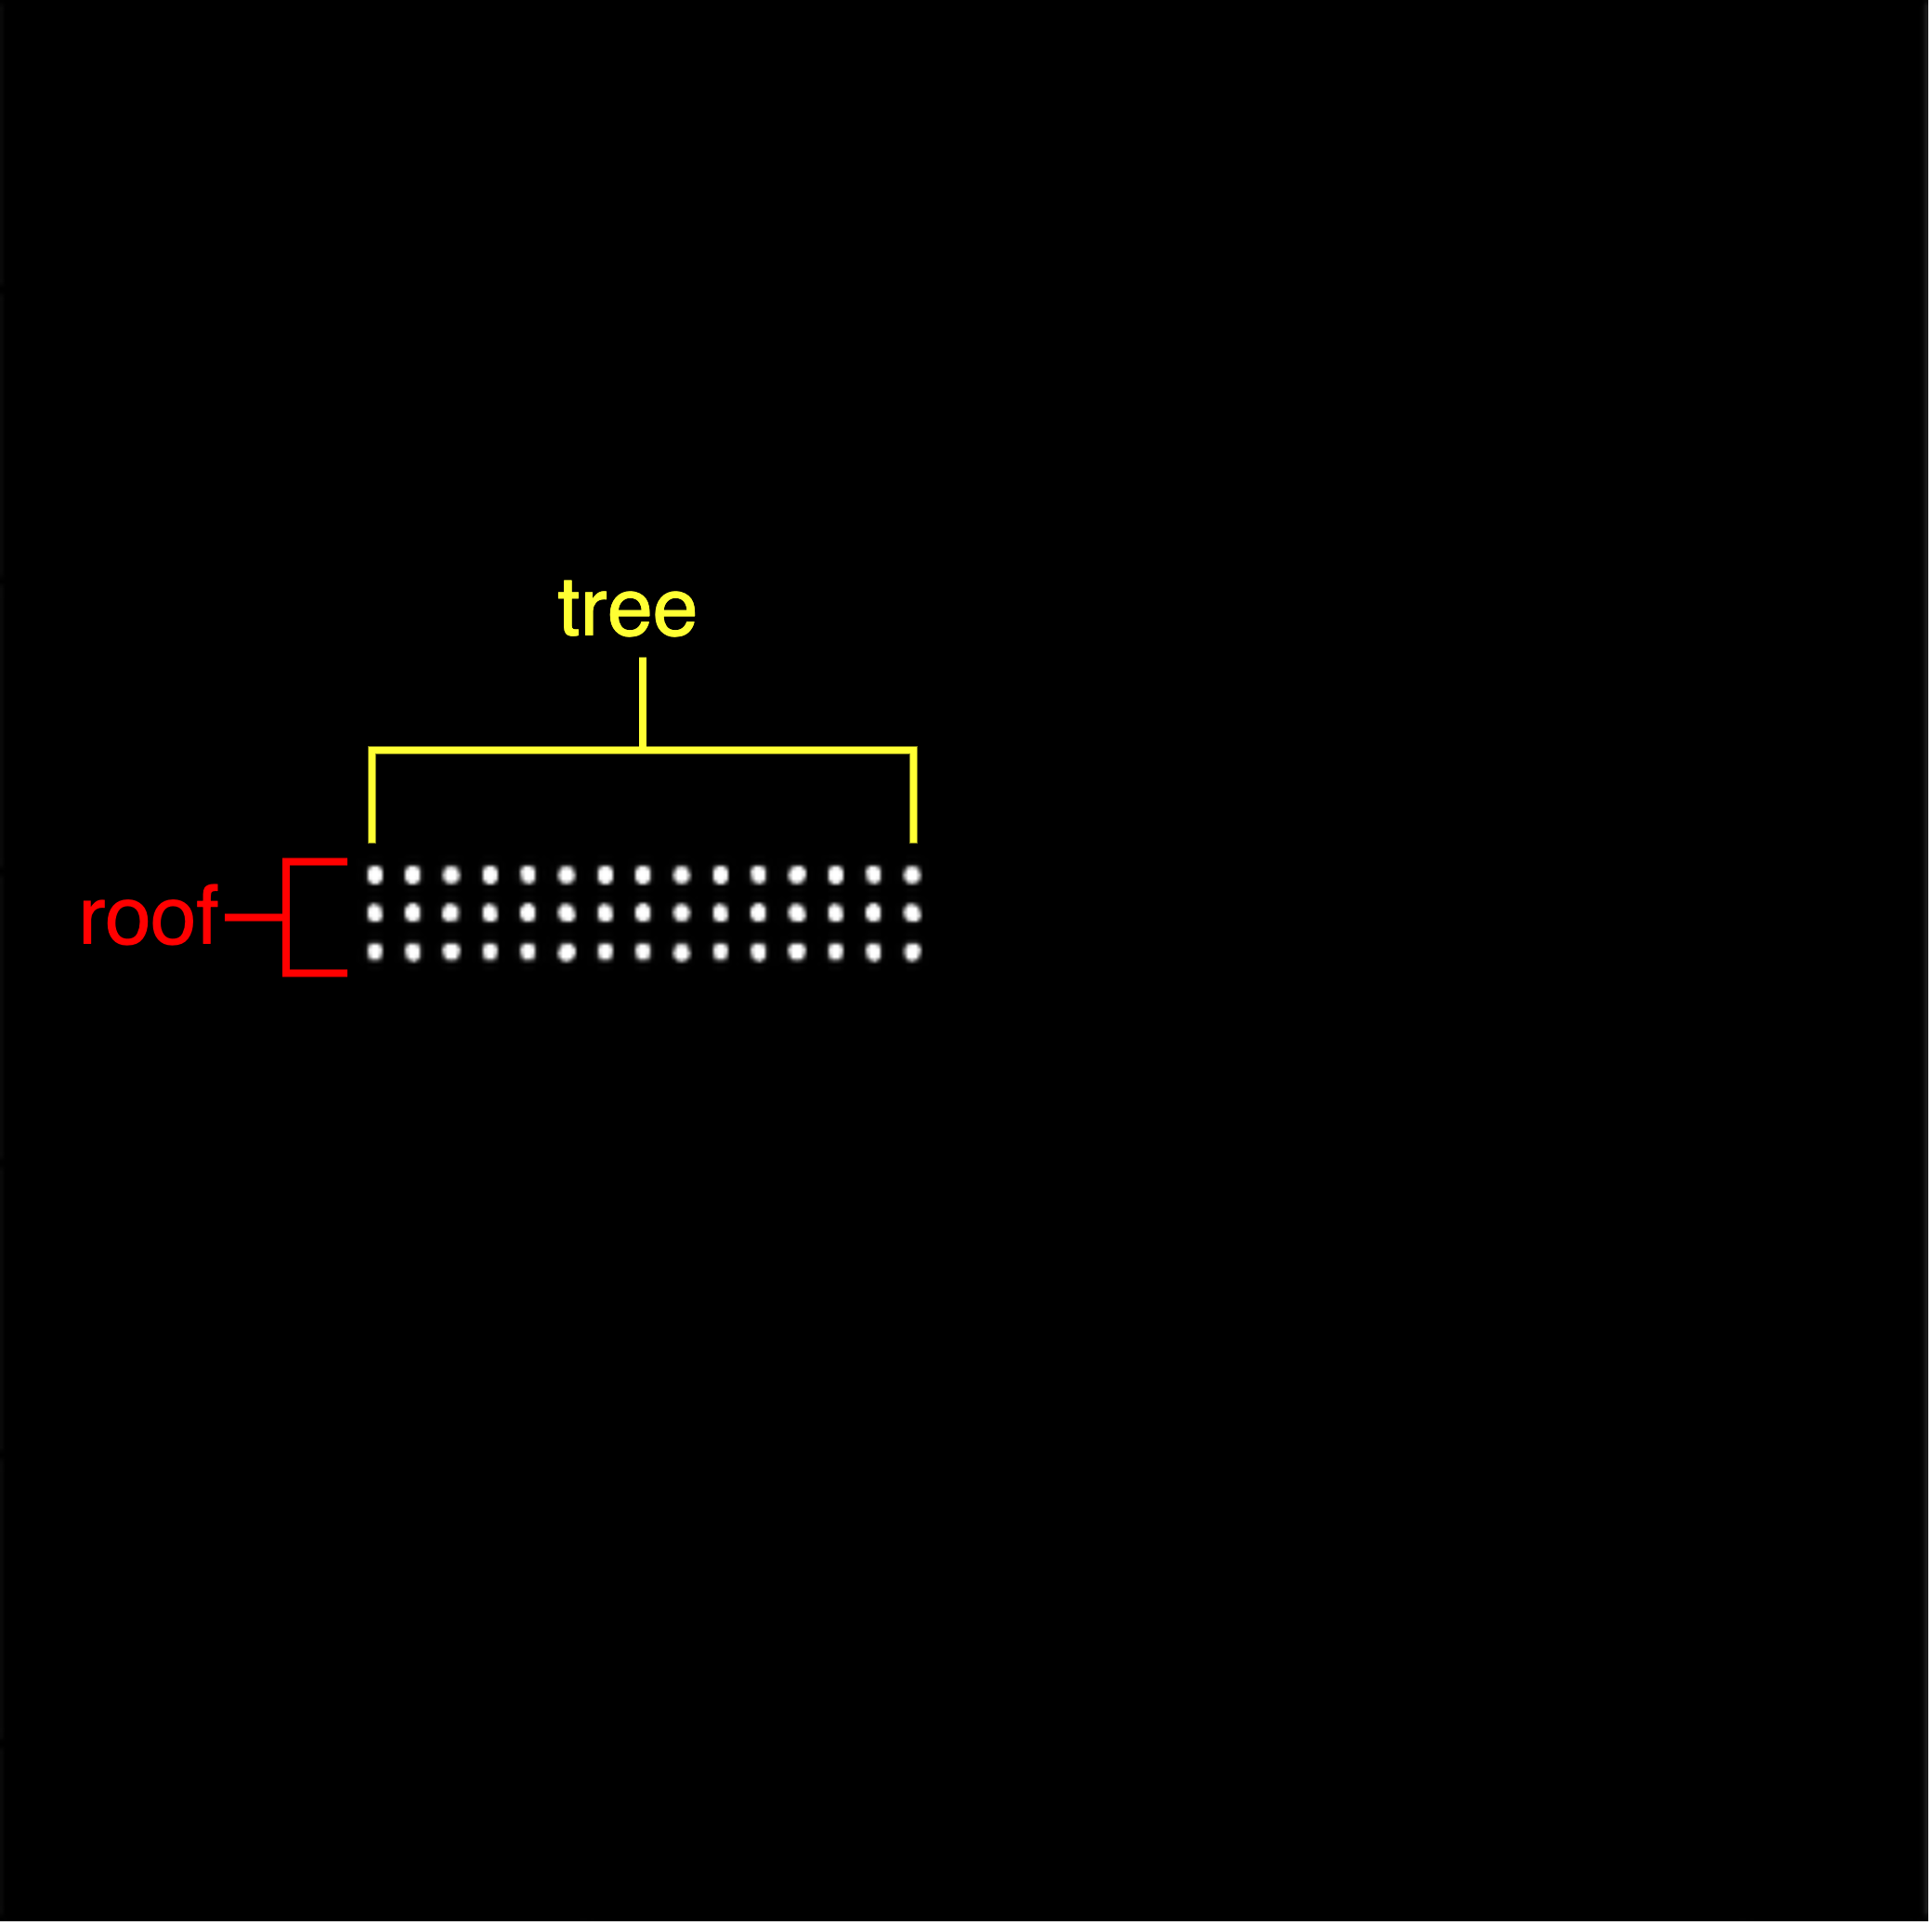
\includegraphics[width=0.8\linewidth]{figures/roof/map1}
	\end{minipage}}
	
	\subfigure[GT relation: \textit{roof on building}.]{
		\begin{minipage}[t]{6cm}
			\centering
			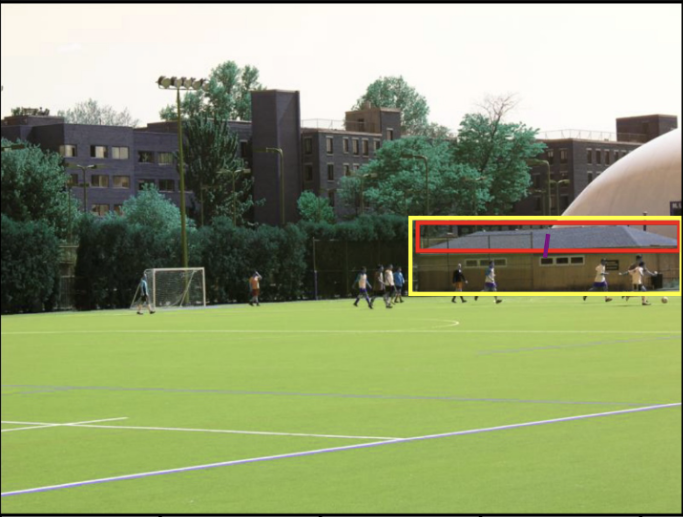
\includegraphics[width=1\linewidth]{figures/roof/img2}
	\end{minipage}}
	\subfigure[The attention of $<roof,building>$]{
		\begin{minipage}[t]{6cm}
			\centering
			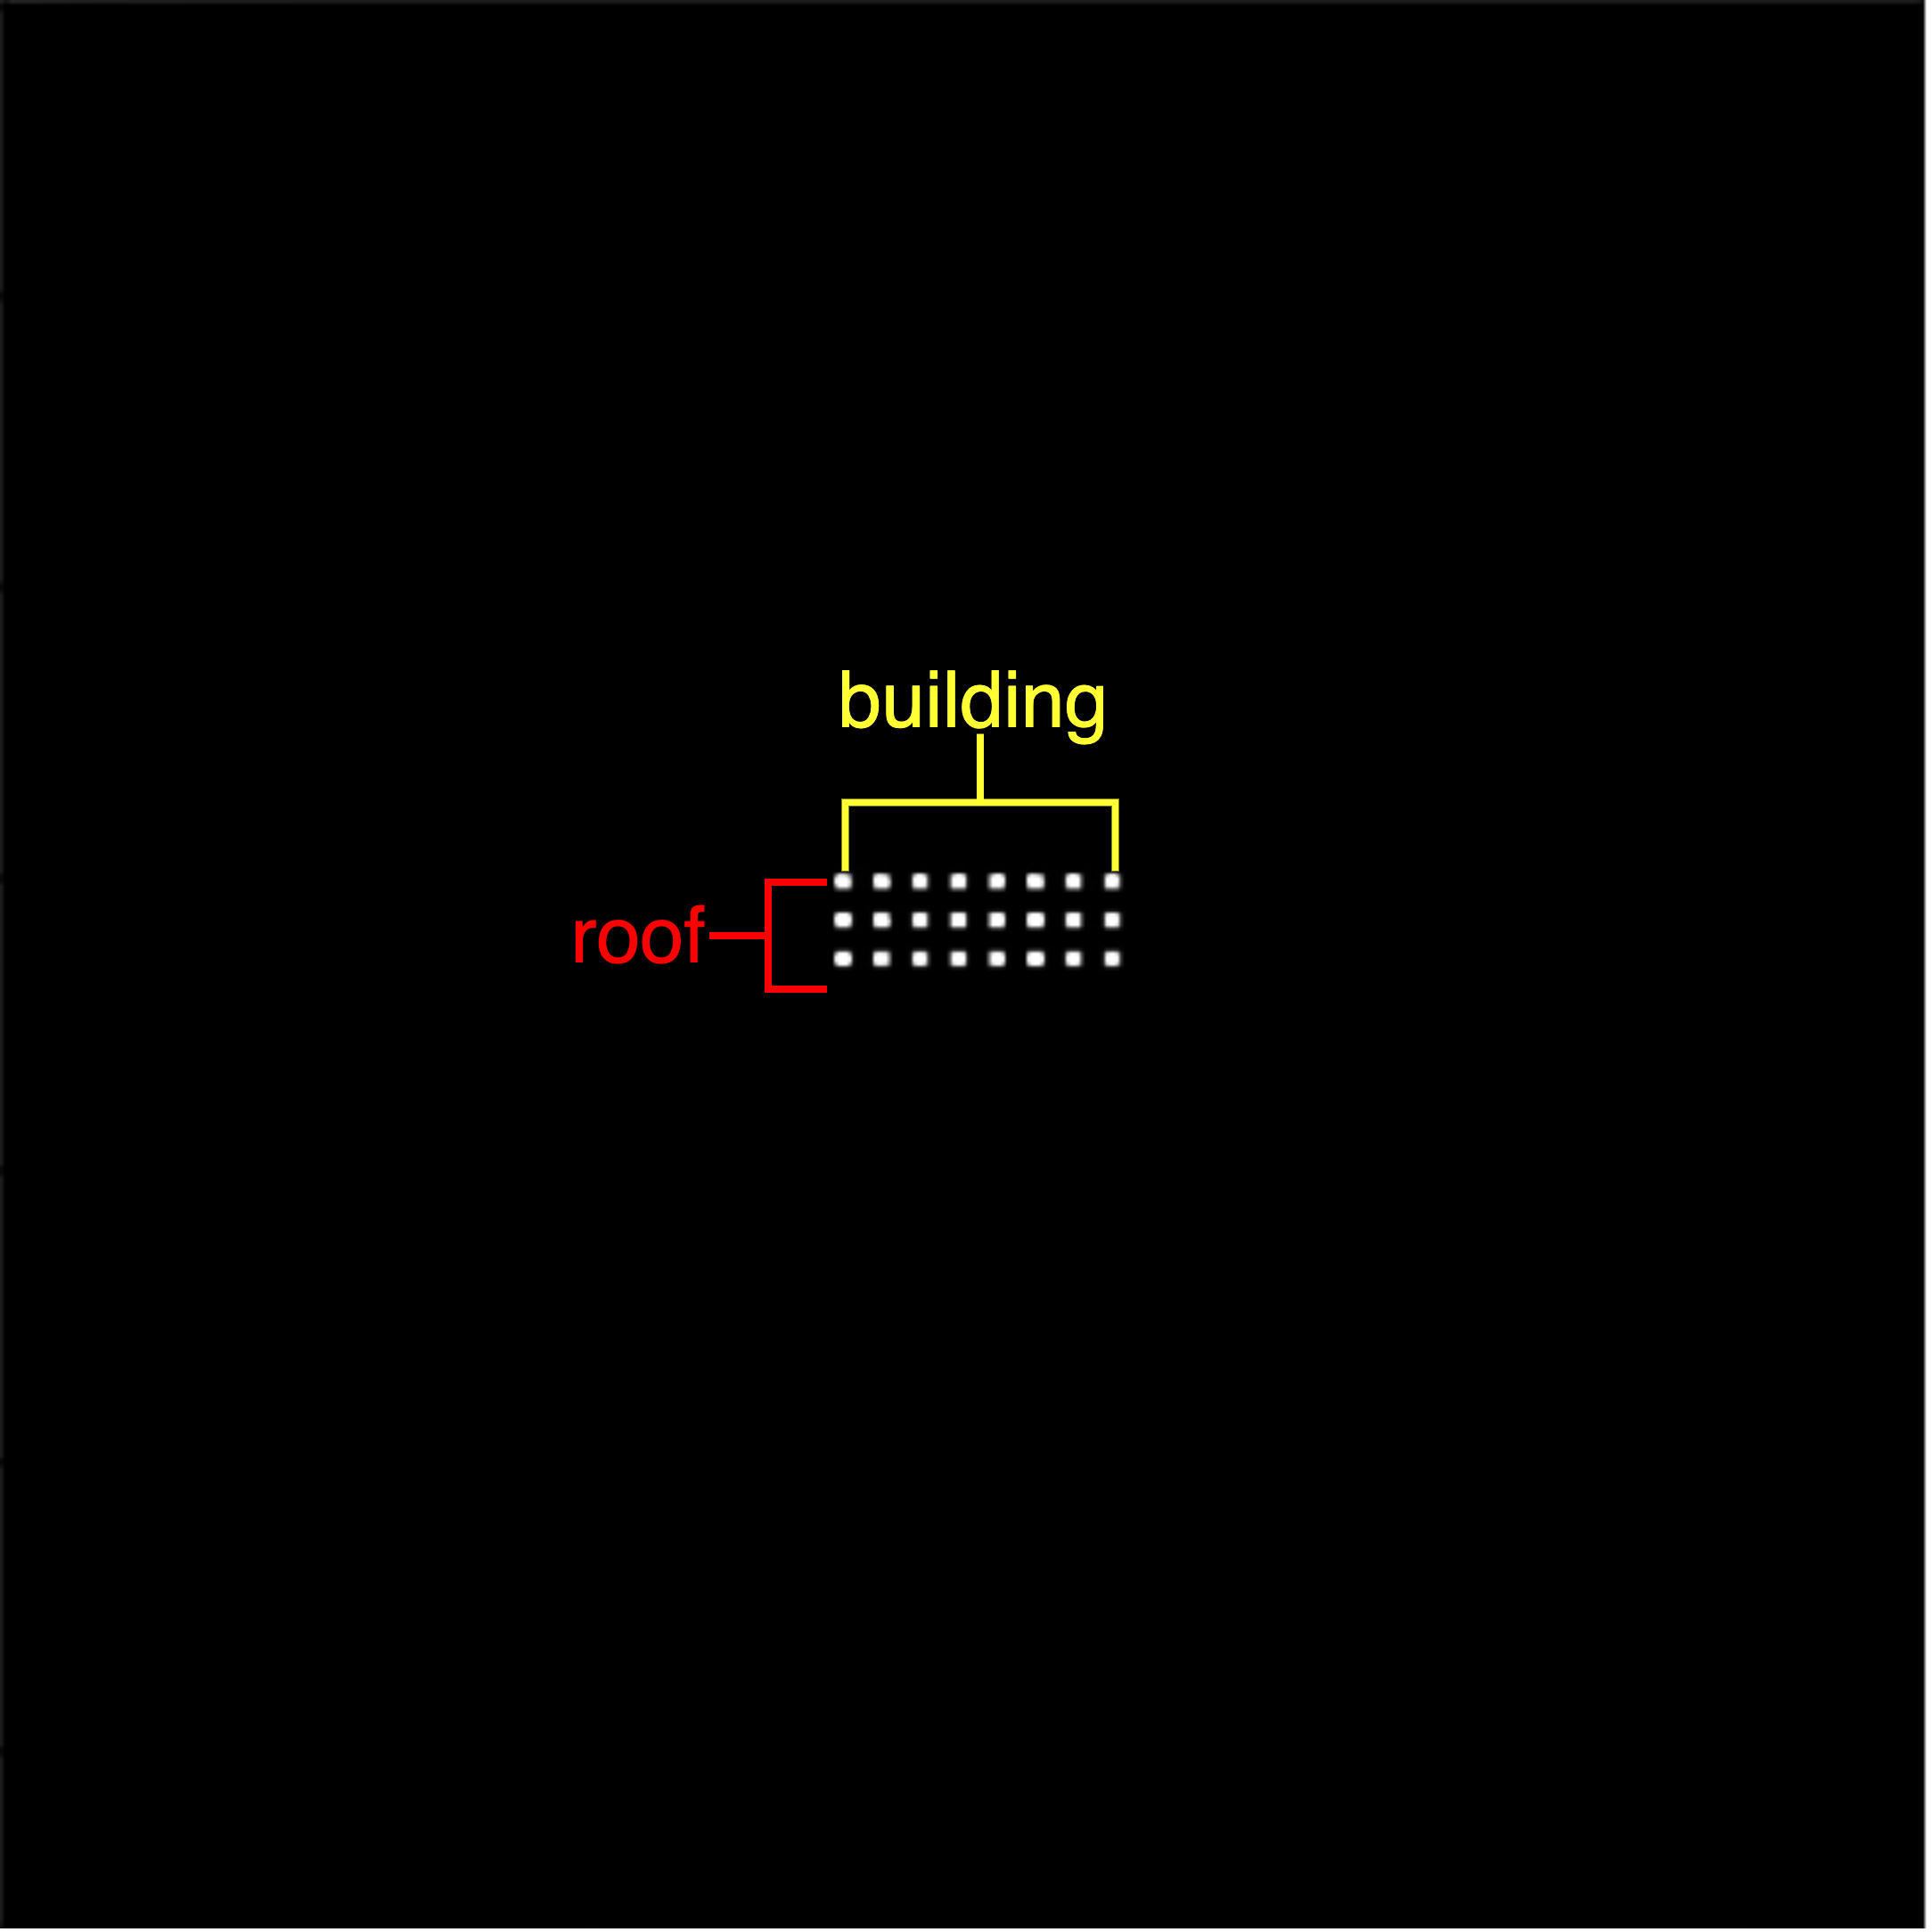
\includegraphics[width=0.8\linewidth]{figures/roof/map2}
	\end{minipage}}

	\caption[An example of Pixel-based attention]{Relation pair on image and its position on attention map.}
	\label{fig:ideamethod1}
\end{figure}

\subsection{ Prototype model}
The concrete realization of our idea is as follows: As shown in following Figure~\ref{fig:method1baseline}, first we input an image into the  backbone VGG16~\cite{simonyan2015deep}(see Figure~\ref{fig:vgg16}.) to gets a down-sampled image feature \textit{feature} ,  then it passes through a Multi-Head Self-Attention module to get an attention map and new image feature \textit{feature2}. Finally, the feature of the subject-predicate object is extracted by ROI Align(see in Section~\ref{fig:roialign}), and sent to the predicate classifier as input.


\begin{figure}[!htbp]
	\centering
	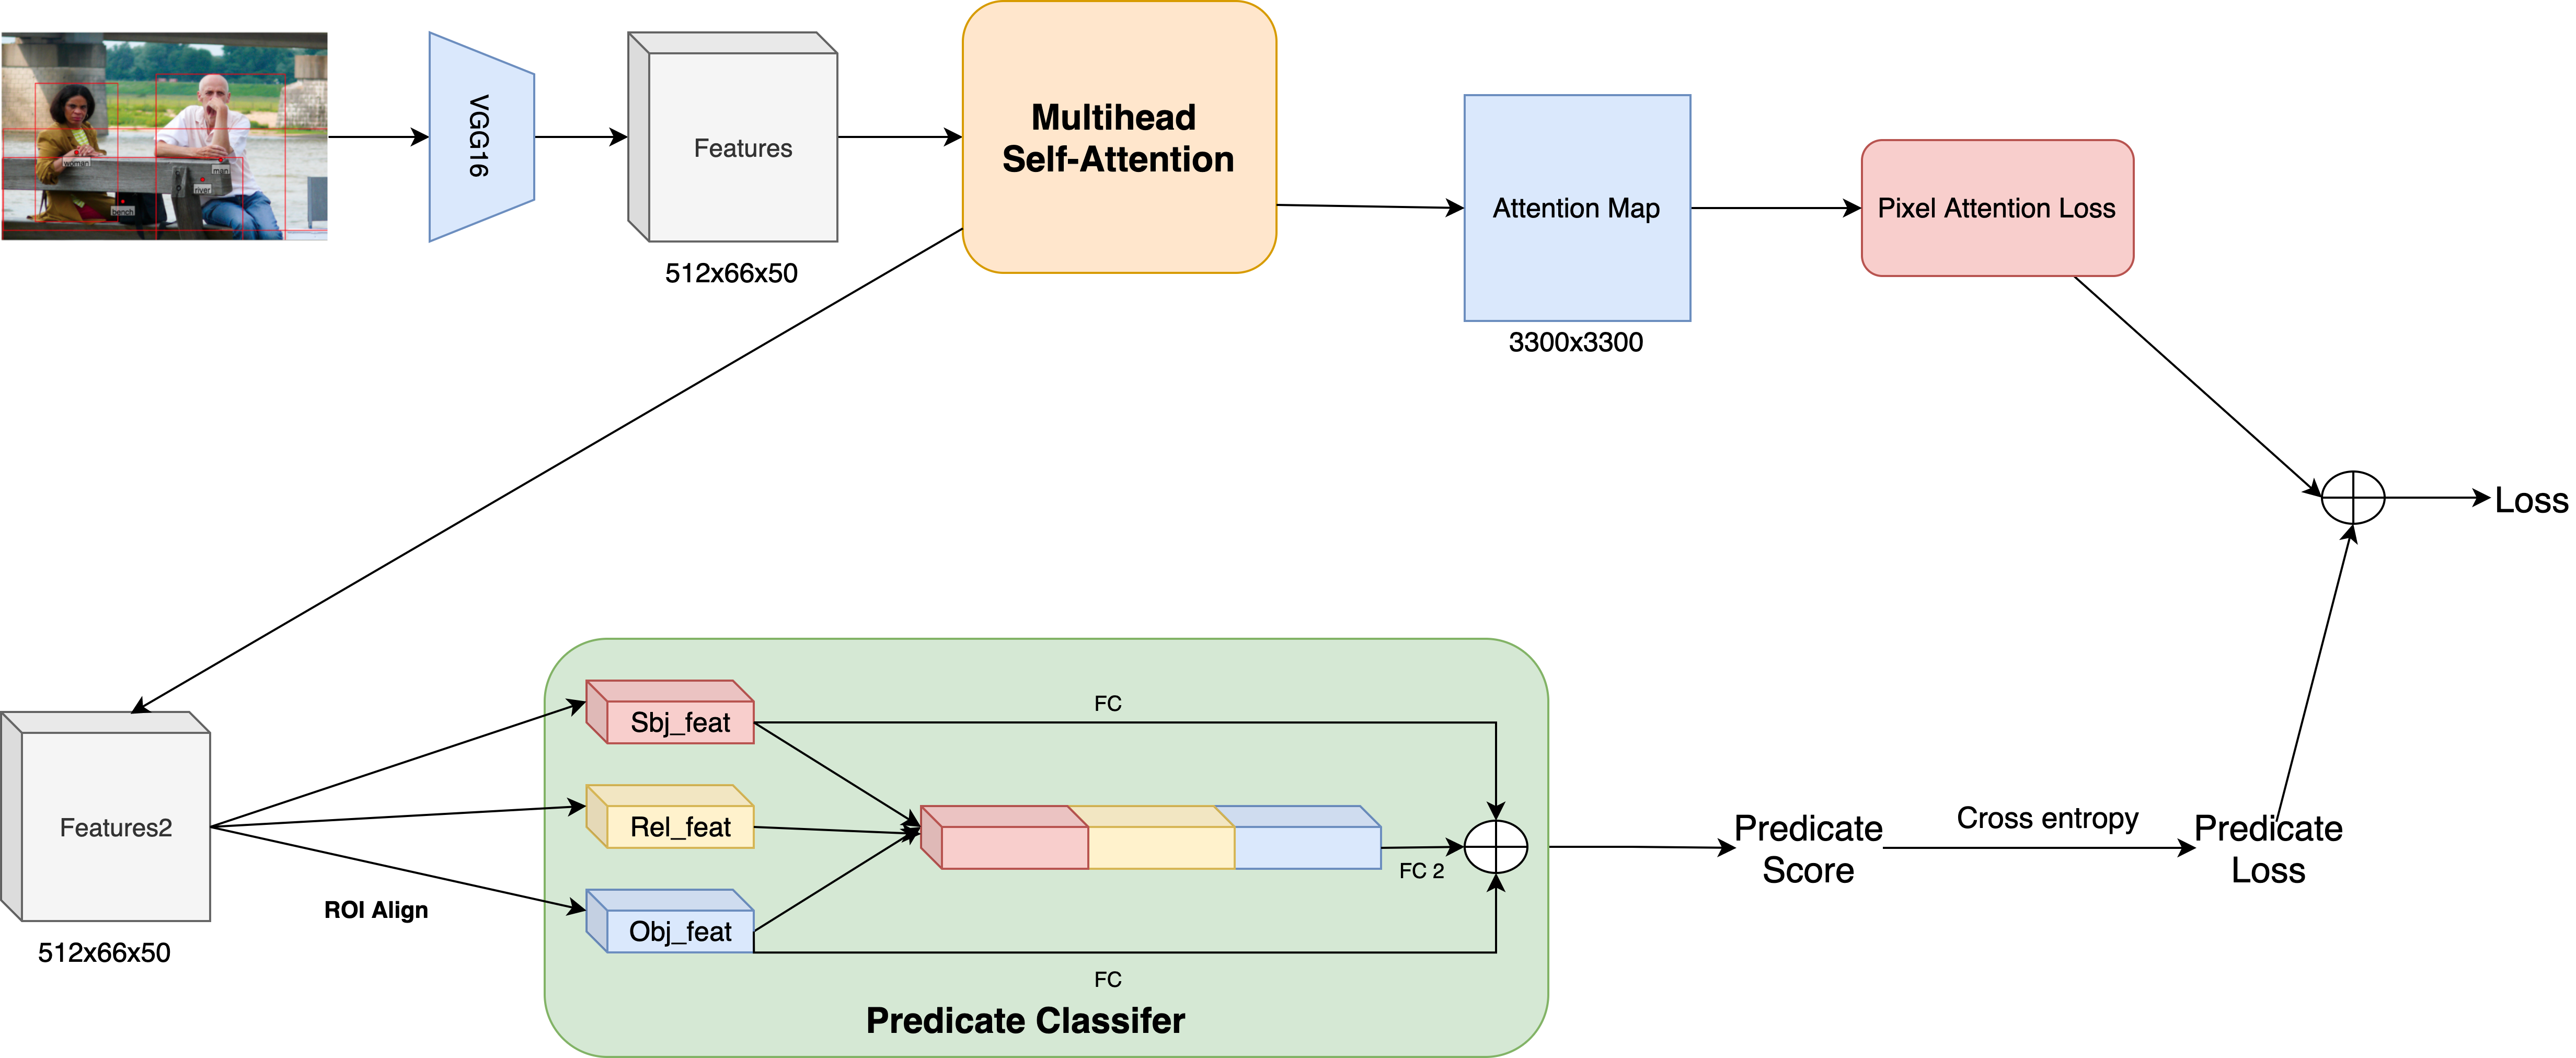
\includegraphics[width=1\linewidth]{figures/method1_baseline}
	\caption[The baseline of the first method: Pixel-based attention]{The baseline of the  first method: Pixel-based attention}
	\label{fig:method1baseline}
\end{figure}

\subsection{Pixel  Attention Loss}

\begin{figure}[htbp]
	\centering
	\subfigure[The relationship between objects.]{
		\begin{minipage}[t]{7cm}
			\centering
			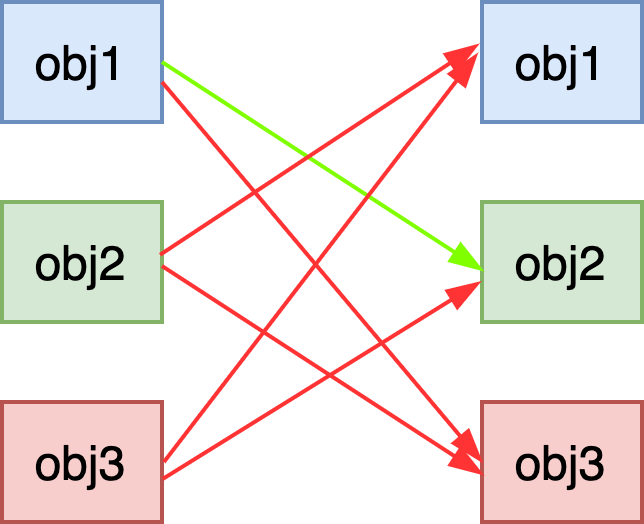
\includegraphics[width=0.8\linewidth]{figures/pixel_relation}
			\label{fig:idea_pixelloss_a}
		\end{minipage}}
	\subfigure[The attention map of each pixel of the image feature.]{
		\begin{minipage}[t]{7cm}
			\centering
			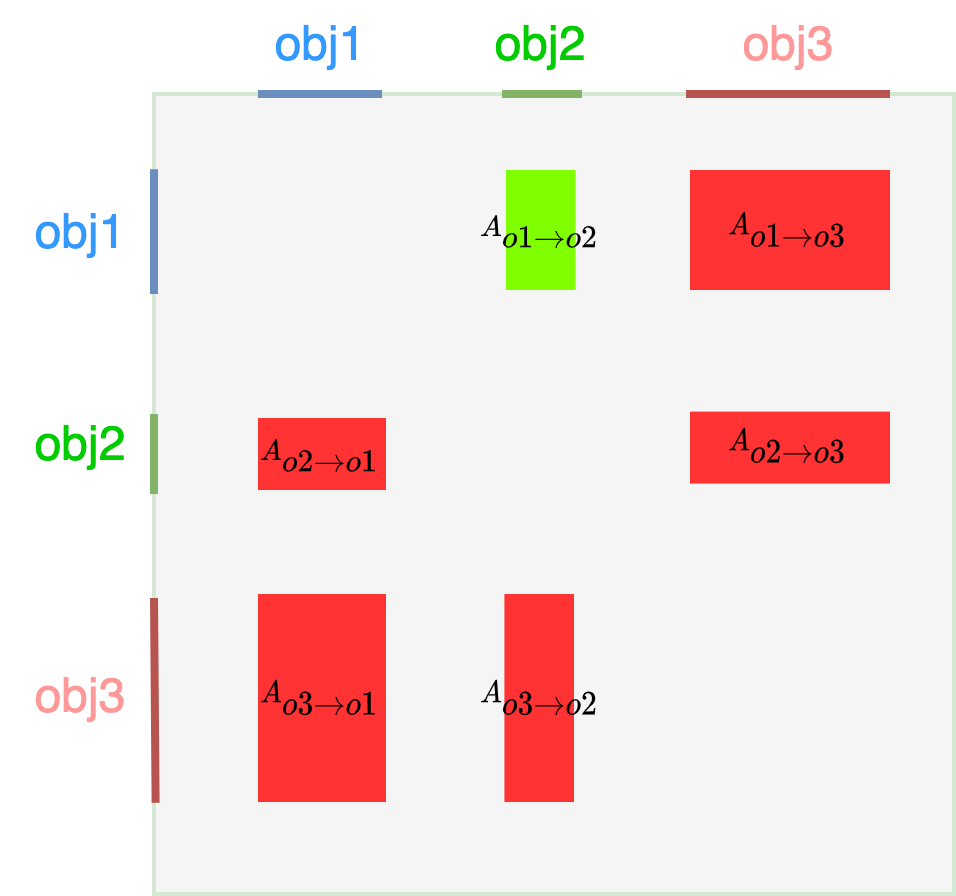
\includegraphics[width=0.9\linewidth]{figures/pixel_attentionmap}
			\label{fig:idea_pixelloss_b}
		\end{minipage}}
	\caption[The idea of the pixel attention loss]{The idea of the pixel attention. The Fig. (a) shows, that there is only relationship between $obj_1$ and $obj_2$(the green line),there are no relationship between the others. The Fig. (b) show the position of the realtion pair. The green area means realtionship, the red area means no relationship. $A_{oi \to oj}$ means the attention weights of the pixel of $obj_i$ to  the pixel of $obj_j$.}
	\label{fig:idea_pixelloss}
\end{figure}

We have studied the attention map, and its meaning is the attention between all pixels of the image feature( $ Attention_{p_i\to p_j}, \  wehre \quad p_i,p_j\in \mathbb{P}_{img} $) , $ \mathbb{P}_{img}  $is a collection containing all pixels of the image feature from VGG16.

We want to know whether $ obj_i  $has a relationship with $ obj_j$ through attention. For example, we have three objects ($ obj_1 $, $ obj_2 $, $ obj_3 $) . Assuming there is a relationship between $ obj_1 $ and $ obj_2 $, $ obj_1 $ and $ obj_3 $, $ obj_2 $ and $ obj_3 $ are not related, see in Fig.~\ref{fig:idea_pixelloss_a}, the green line means $ pair <obj_1,obj_2> $ has relationship, while the red line means the other pairs have no relationship. 

We first have the following definition: 
$$ Attention_{p_{obj_i}\to p_{obj_j}},\ where \quad p_{obj_i} \in \mathbb{P}_{obj_i},\  p_{obj_j} \in \mathbb{P}_{obj_j} $$
Where $ \mathbb{P}_{obj_i}, $ represents the collection of all pixels of $ obj_i $ on the image feature obtained from VGG16. $  Attention_{p_{obj_i}\to p_{obj_j}} $ means the attention weight between the pixel $ p_{obj_i} $ and the pixel $ p_{obj_j} $. In Fig.~\ref{fig:idea_pixelloss_b} we abbreviate it as $ A_{oi \to oj} $. and we can see the green area means there is a relationship.



we want to know which pair is more relevant in evaluation through the attention weights between each pixel on the down-sampled image feature, thus we design a pixel attention loss as following:
\begin{equation}\label{pixel_attention_loss}
	loss_{attention}=max(0, \frac{1}{m}\sum_{m}Att_j^{no\_rel}-\frac{1}{n}\sum_{n}Att_i^{rel}+0.25
	/3300)
\end{equation}

Where:

\begin{itemize}
	\item $ Att_j^{no\_rel} $ : the attention weight of the pixel j of no-relation pairs.
	\item $ Att_i^{rel} $ :  the attention weight of the pixel i of gt relation pairs.
	\item Margin=0.25/3300 is quarter the average of the attention map.
\end{itemize}

For example, in Fig.~\ref{fig:idea_pixelloss_b} , our $Att_i^{rel} $  is $ A_{o1 \to o_2} $ (the green area) and  the $ Att_j^{no\_rel} $ are $ A_{o1 \to o_3}  $,  $ A_{o2 \to o_1}  $, $ A_{o2 \to o_3}  $, $ A_{o3 \to o_1}  $ and $ A_{o3\to o_2}  $(the red areas). We use our attention loss to make attention weights of the green area in this figure higher and the value of the red area lower. In this way, we can judge which can have a relationship through the attention value of each pair during evaluation.

For this method, we have conducted many attempts and experiments. Through our experimental verification, we found that the results did not achieve our expectations. After thinking, we found a very serious problem. For the specific experimental results and analysis, please refer to the following chapters. So we changed our thinking, changed from pixel-based to box-based, and used the complete transformer encoder decoder structure, and added our own design here. Next we will introduce our final model Retina Net.

\section{Retina Net}
\label{sec:retinanet}
After previous trial and error, we changed our thinking and proposed our new model structure Retina-Net.we completed the three tasks of the VRD problem: \textit{predicate classification} , \textit{scene graph classification} and \textit{scene graph detection} . For these three tasks, our model is unified, based on the transformer model, and other parts such as the decoder for the relationship have been added.

In our Framework (see Fig.~\ref{fig:my_model}), we propose a new visual relationship detection network, our network consists of a convolutional neural network (CNN) backbone, an \textit{Encoder} module, \textit{Object Decoder} module to obtain object features and  the context between each entity, \textit{Relation Decoder} module to obtain the context beween entities and relation  , and a \textit{Predicate Classifer} module to predict predicate.

\begin{figure}[!htbp]
	\centering
	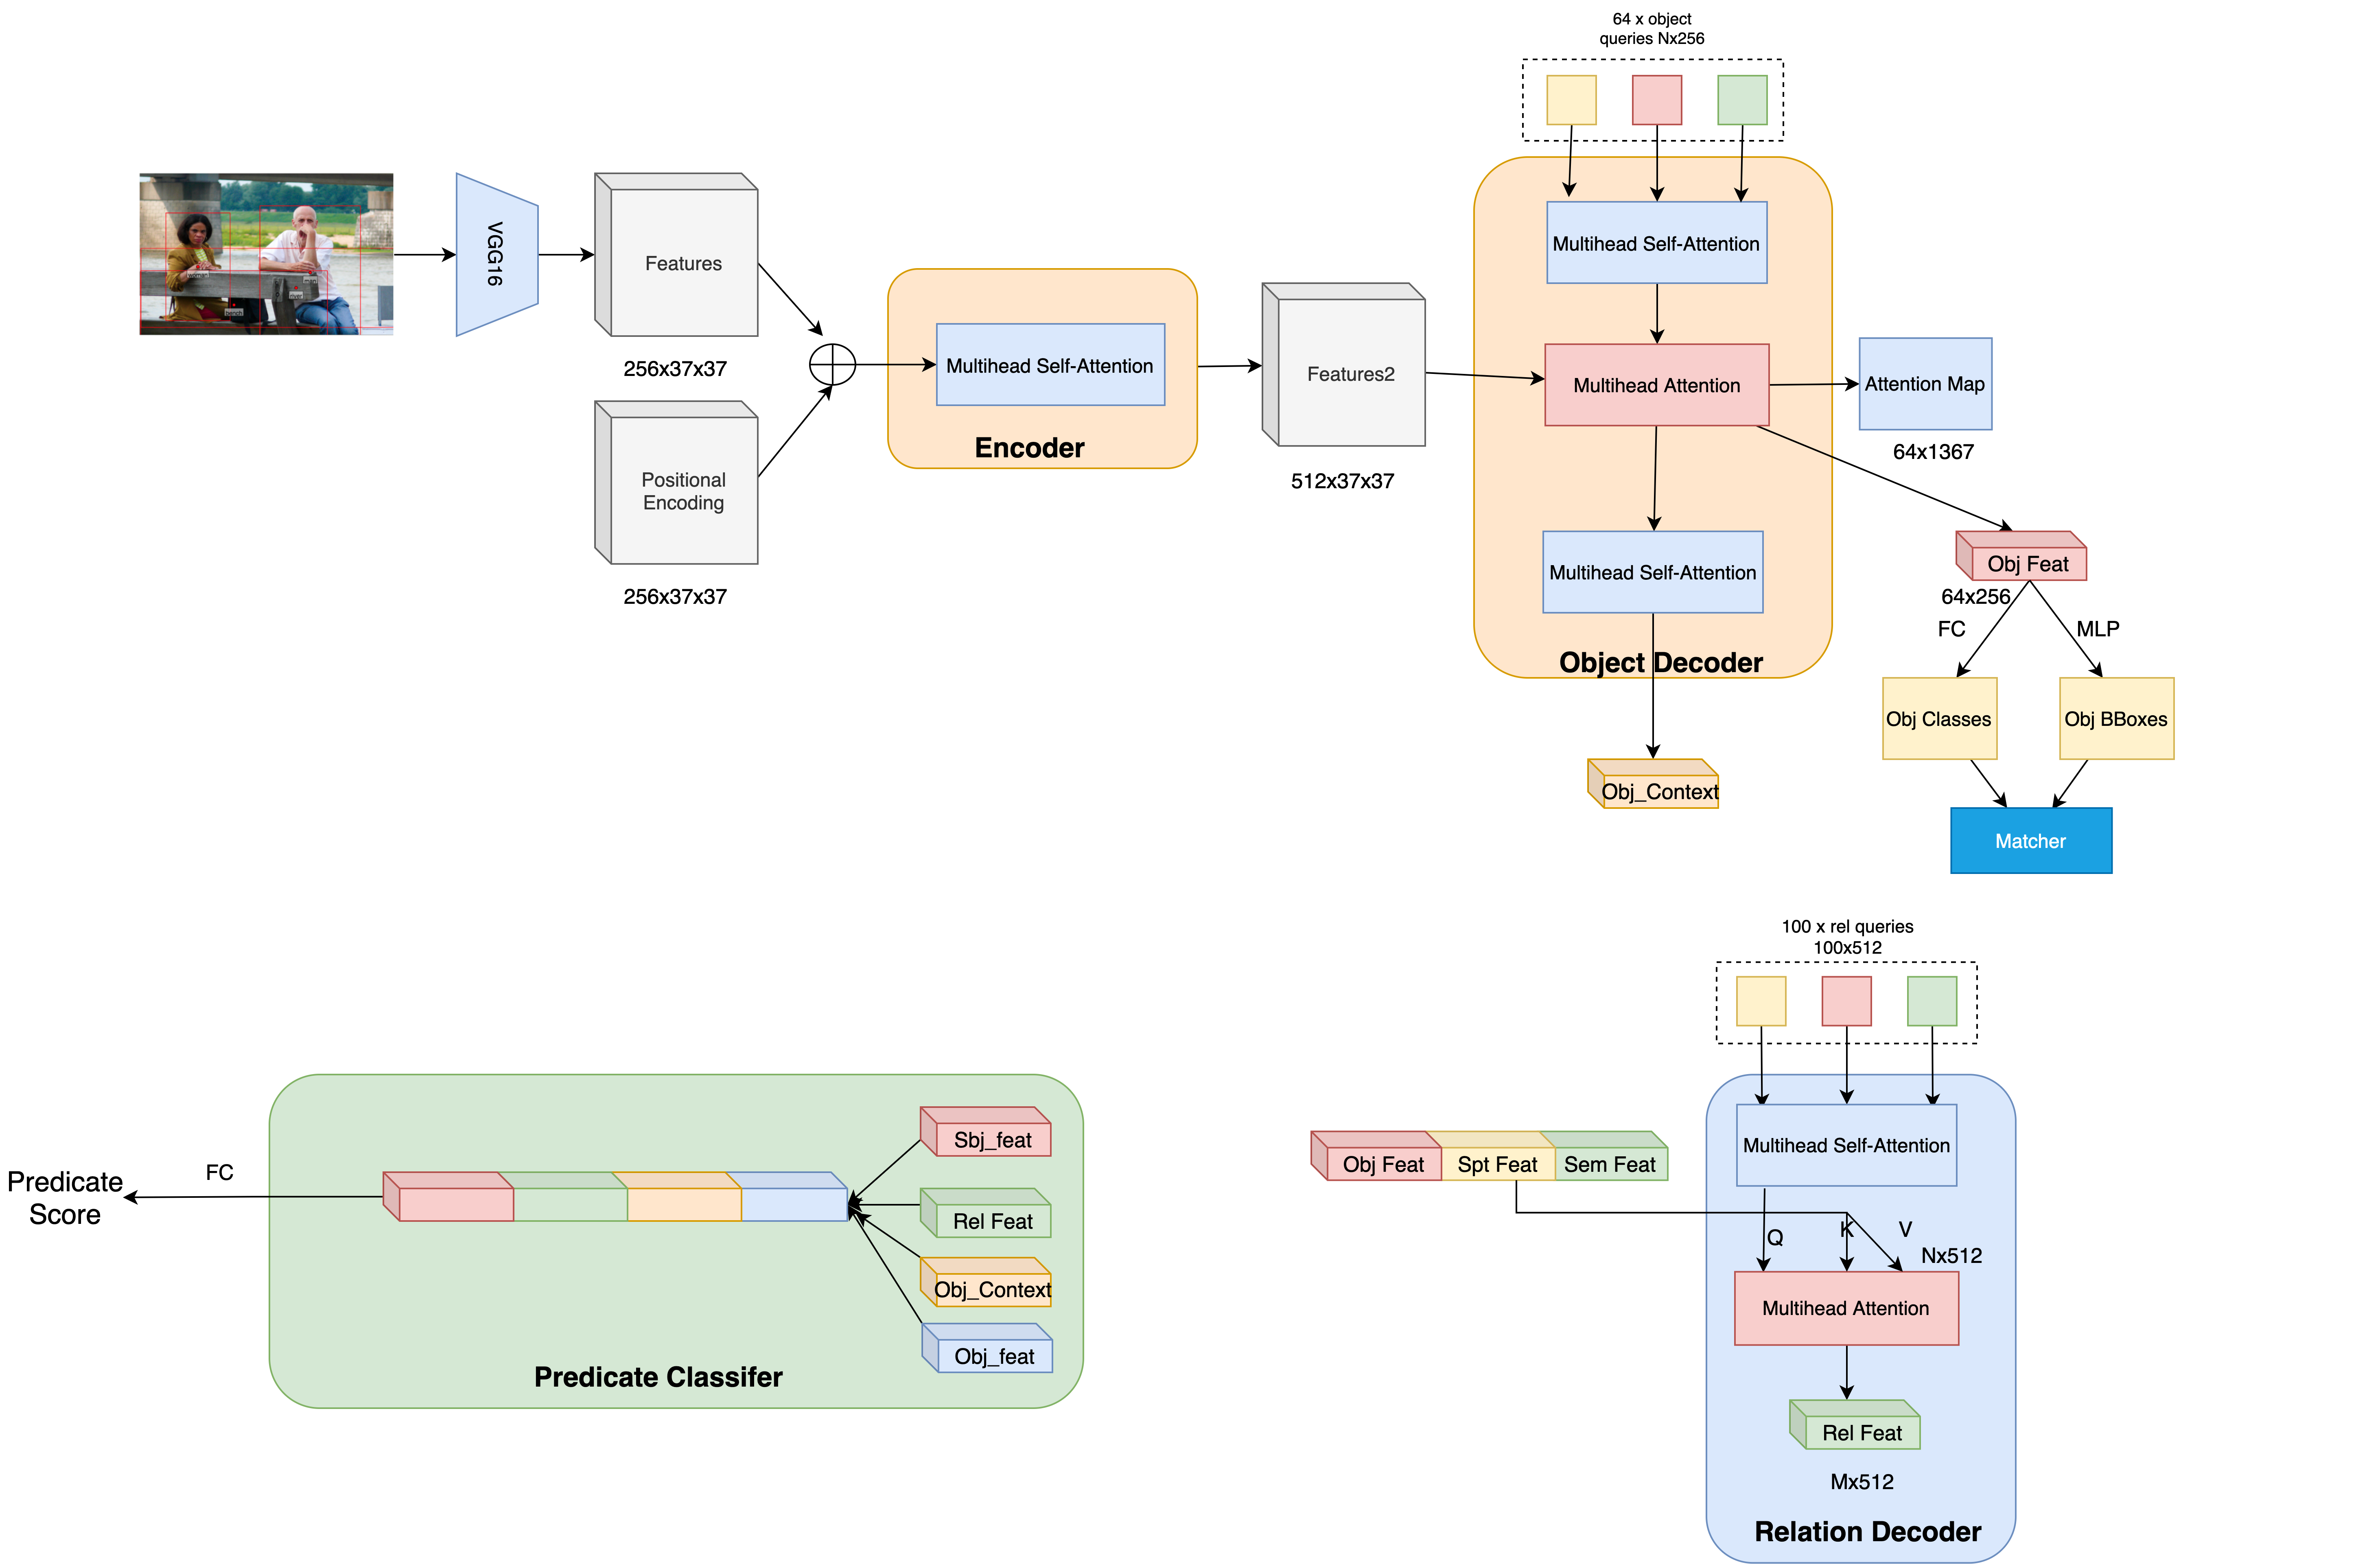
\includegraphics[width = 1\textwidth]{figures/my_model.png}
	\caption[The architecture of our model.]
	{The architecture of our model,it consists of a convolutional neural network (CNN) backbone, an Encoder, an Object Decoder, a Relation Decoder and a Predicate Classifier.}
	\label{fig:my_model}
\end{figure}


\subsection{Generation of Image Feature Maps }

We first use vgg16 to extract preliminary image features, and then generate a final image feature through an Encoder(see in Fig.~\ref{fig:imgfeatbaseline}).

In the proposed framework the VGG16 as backbone is used to extract preliminary feature maps $f^{vgg}_{img}$ and  then generate final image features $f^{en}_{img}$ through an Encoder. Before an image is fed into the VGG16 net it is rescaled and zero padded to a Tensor with the size $ 3\times592\times592 $. Then the scaled image is normalized with $ mean = [0.485, 0.456, 0.406 ]$ and $ std = [ 0.229, 0.224, 0.225]$.   The size of feature $f^{vgg}_{img}$ is $512 \times 37 \times 37$. Before we input it into the encoder, we need to convert $f^{vgg}_{img}$  into a sequence tensor.In order to reduce the parameter size, we set the size of the sequence element to 256, that is, the number of feature layers is changed from the original 512 to 256, so we need to add a convolutional layer between vgg16 and the encoder, whose stride and kernel size are both 1. Finally we will set the size to $ 1369 \times bs \times 256 $, where $ 1369 $ is the sum of down-sampled pixels of each layer in image feature $f^{vgg}_{img}$ ($ 37 \times 37 = 1369$), $ bs $ is our batch size, and $ 256  $is the size of the feature of each sequence. The size of the output feature $f^{en}_{img}$ is same as that of the input ($ 1369 \times bs \times 256 $), we can also reshape the output to the size of $256 \times 37 \times 37$.


\begin{figure}[tbph!]
	\centering
	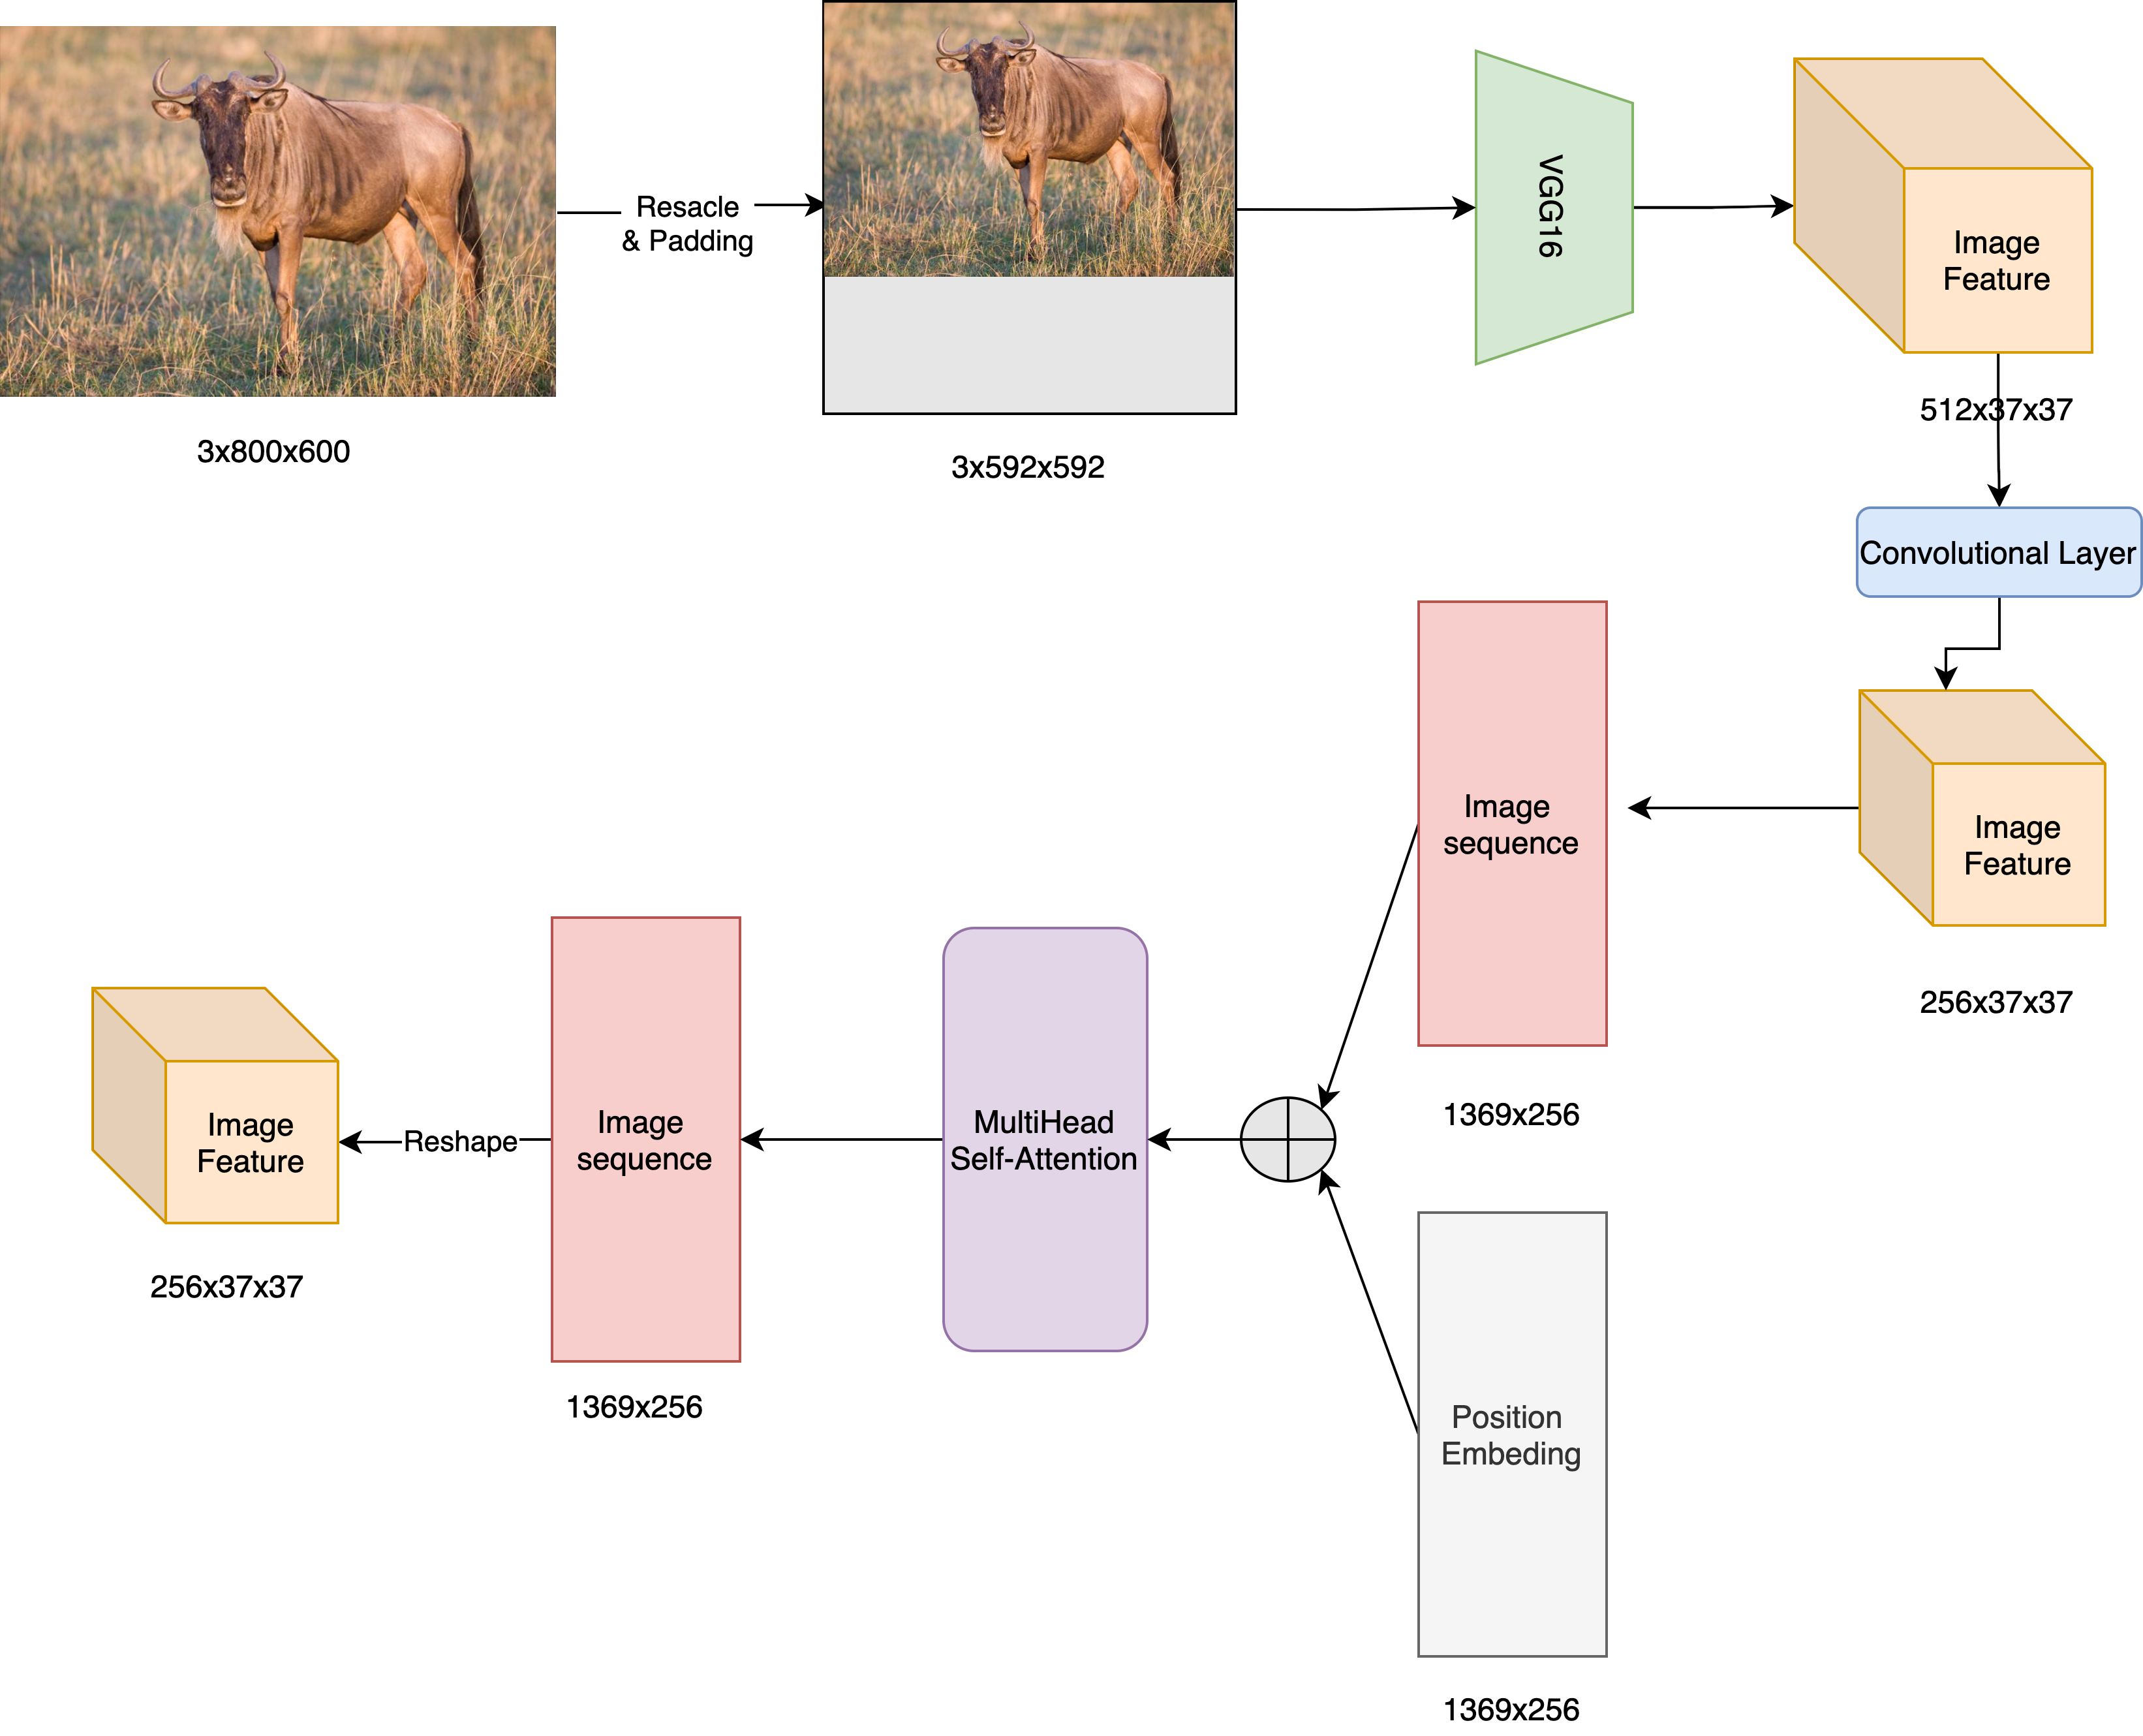
\includegraphics[width=0.9\linewidth]{figures/img_feat_baseline}
	\caption[Generation of Image Feature Map]{Illustration of the generation of image feture map.}
	\label{fig:imgfeatbaseline}
\end{figure}


Ours Encoder is a MultiHead Self-Attention module, whose input is an image sequence tensor plus a  Position Embedding tensor. Different from the processing of sequence signals by the RNN network, the Self-Attention module processes the sequence in parallel, so it does not know the order of the sequence, we need to add position information to the original sequence.  we are processing two-dimensional image information, thus we need to add two-dimensional position information for each pixel. We use Equ.~\ref{equ:position_embedding} to encode the position of the picture pixels.


\subsection{Object Decoder }

In this part we will introduce a very important part of the model: \textit{Object Decoder}. We use a custom object query to obtain the object feature and context between each entity through three Multihead Attention models(see Fig.~\ref{fig:objectdecoder}).

\begin{figure}[tbph!]
	\centering
	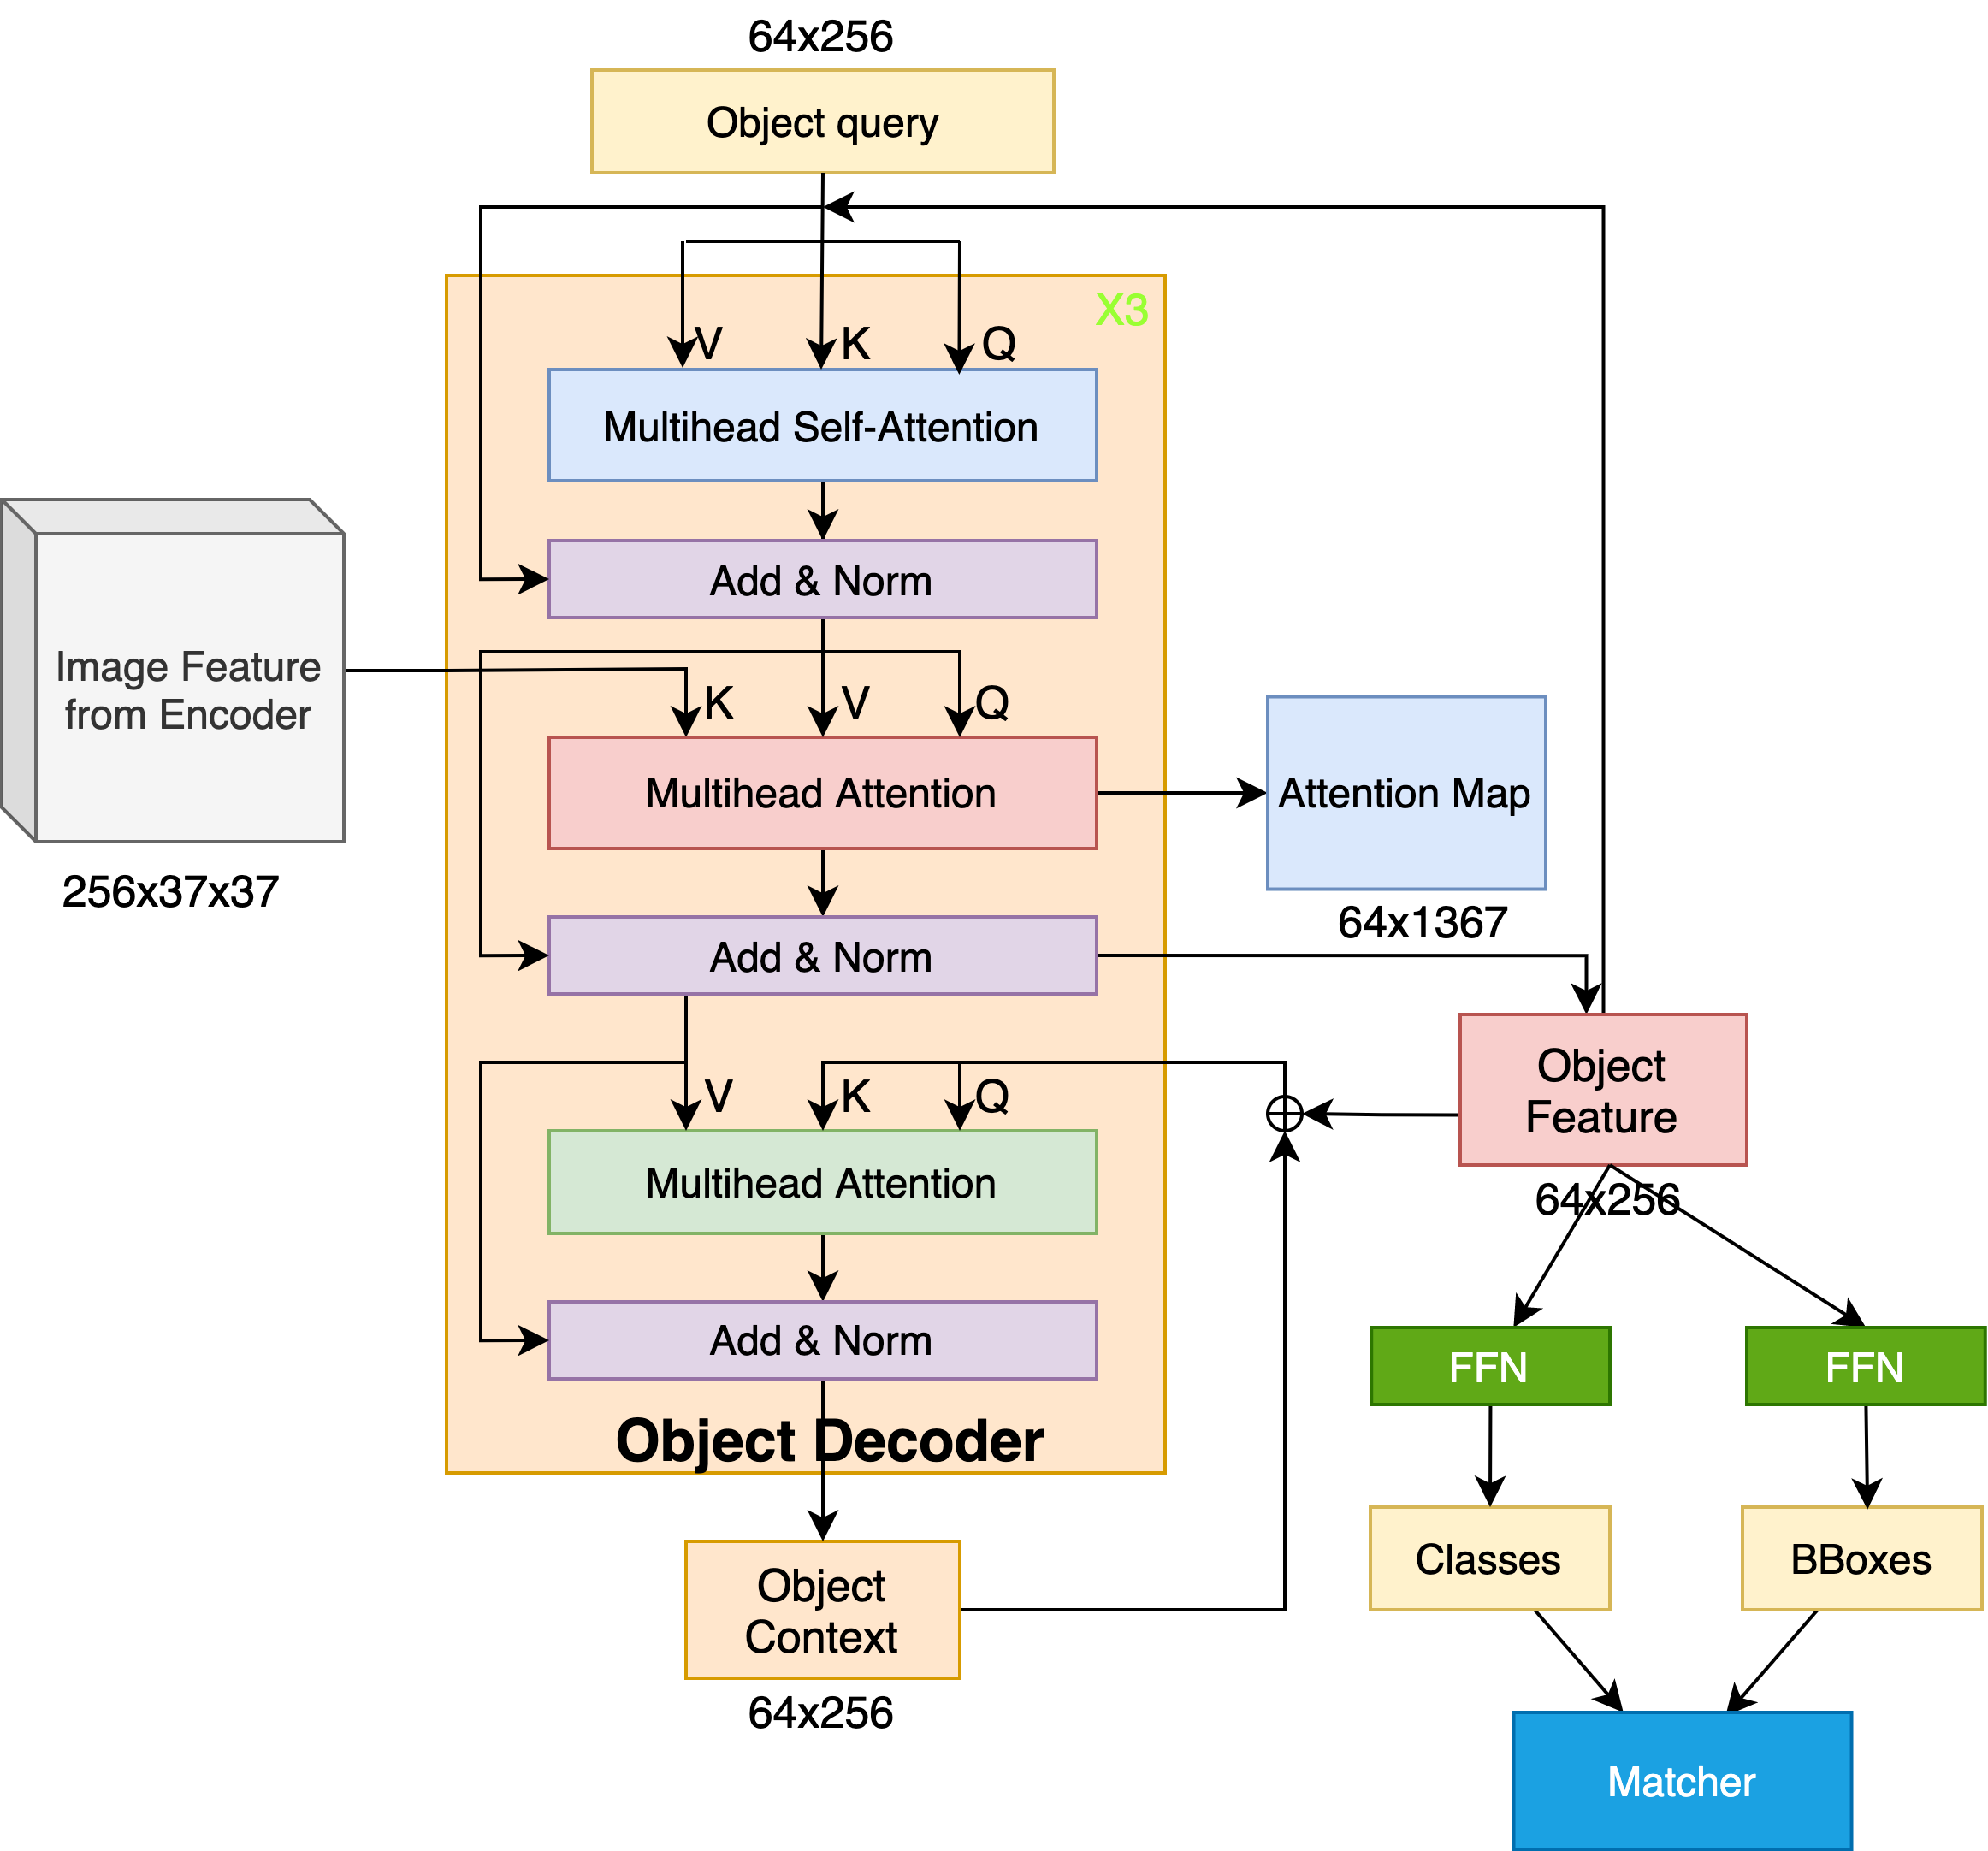
\includegraphics[width=0.9\linewidth]{figures/object_decoder}
	\caption[Illustration of the Object Decoder]{The architecture of the Object Decoder, it consists of three Multihead Attention modules,it can obtain three outputs, Attention Map, Object Feature and Object Context.}
	\label{fig:objectdecoder}
\end{figure}

%\subsubsection{The overview of Object Decoder}
As shown in Figure~\ref{fig:objectdecoder}, our decoder structure is similar to the decoder structure in the traditional transformer~\cite{vaswani2017attention}. The difference is that we added a new Multihead Attention  (see the light green part in  Figure~\ref{fig:objectdecoder}). module after the second MultiHead Attention module. In addition, we adopted the Multihead Attention of 8 heads 3 layers. We have also made changes to the object query, which we will explain in detail in the following part.

%We obtained the object feature and an attention weight map in the second Multihead Attention module (see the red part in the middle of Figure~\ref{fig:objectdecoder}). Obtain the object context through the third Multihead Attention module. This means the context of one entity to other entities. For example, we have 10 object entities in a picture. The attention map generated by the second Attention module is the effective part of $ 10 \times 10 $. Of course, the size of the attention map should be $  64\times 64 $ showed in Fig.~\ref{fig:objectdecoder}, but we only have 10 valid entities and the other 54 will be filled with 0 .So the attention map will have an effective part of $ 10 \times 10 $. Its meaning is the attention weight of an entity to other entities, including itself, that is, we have obtained a global context.It is worth mentioning that in the first layer of the Object Decoder operation, we initialize the object context to all zero tensor.


%%We can simply derive each output through Equ.~\ref{equ:self_attention}. We set the image feature from encoder be $f_{img}$, the Object Feature is $ f_{obj} $ ,the object context is $ C_{obj} $, and the attention map from the seconde Attention module is$  Att $.




\subsubsection{Object query}
In related papers (such as DETR~\cite{carion2020end} and Deformable DETR~\cite{zhu2021deformable}), using transformers for object detection, in addition to only one picture information, it is necessary to make predictions of classes and bounding boxes, so they use the learnable obeject query: they used the weight of an embedding layer as the object query. First of all, the interpretability of this query is very poor and has no actual physical meaning. Moreover, in the three tasks of VRD: SGCLS provides the entity's bounding box information, and even the PREDCLS task provides category information. Therefore, in these two tasks, we can make full use of the known information and propose a new entity encoding method to use as an object query.Since the known conditions provided by the three tasks of VRD are not the same, we use different queries.


In this thesis, we propose a custom object query for PREDCLS and SGCLS tasks, as shown in Fig.~\ref{fig:objectquery}. In these two tasks, the bounding box is known information, so we first project the box information of the form $ (x1y1x2y2)  $(where$ [x1,y1] $ is the coordinate of the upper left corner of the box, and $ [x2,y2] $ is the coordinate of the lower right corner of the box)on a size of $ 37 \times 37 $ mask. We set the selected area(the orange area in the figure) be $ 0.5  $ and the unselected area (the yellow area in the figure) be $ -0.5 $. After extracting spatial information through a convolutional layer, the max pooling layer scales the tensor size, and finally transforms it to the size we need $ 64 \times 256 $ through a linear layer.

For the task SGDET, we do not have the information of the bounding box, so we continue to use the learnable object query, that is, use the weight of an embedding layer with a size of $ 64 \times 256 $.

For the size of the object query, we chose $ 64 \times 256 $, because according to our statistics on our dataset, each image has a maximum of 62 bounding boxes, and it has an average of 11.87. So we choose 64 queries will be greater than the maximum number of the entity. 

\begin{figure}[tbph!]
	\centering
	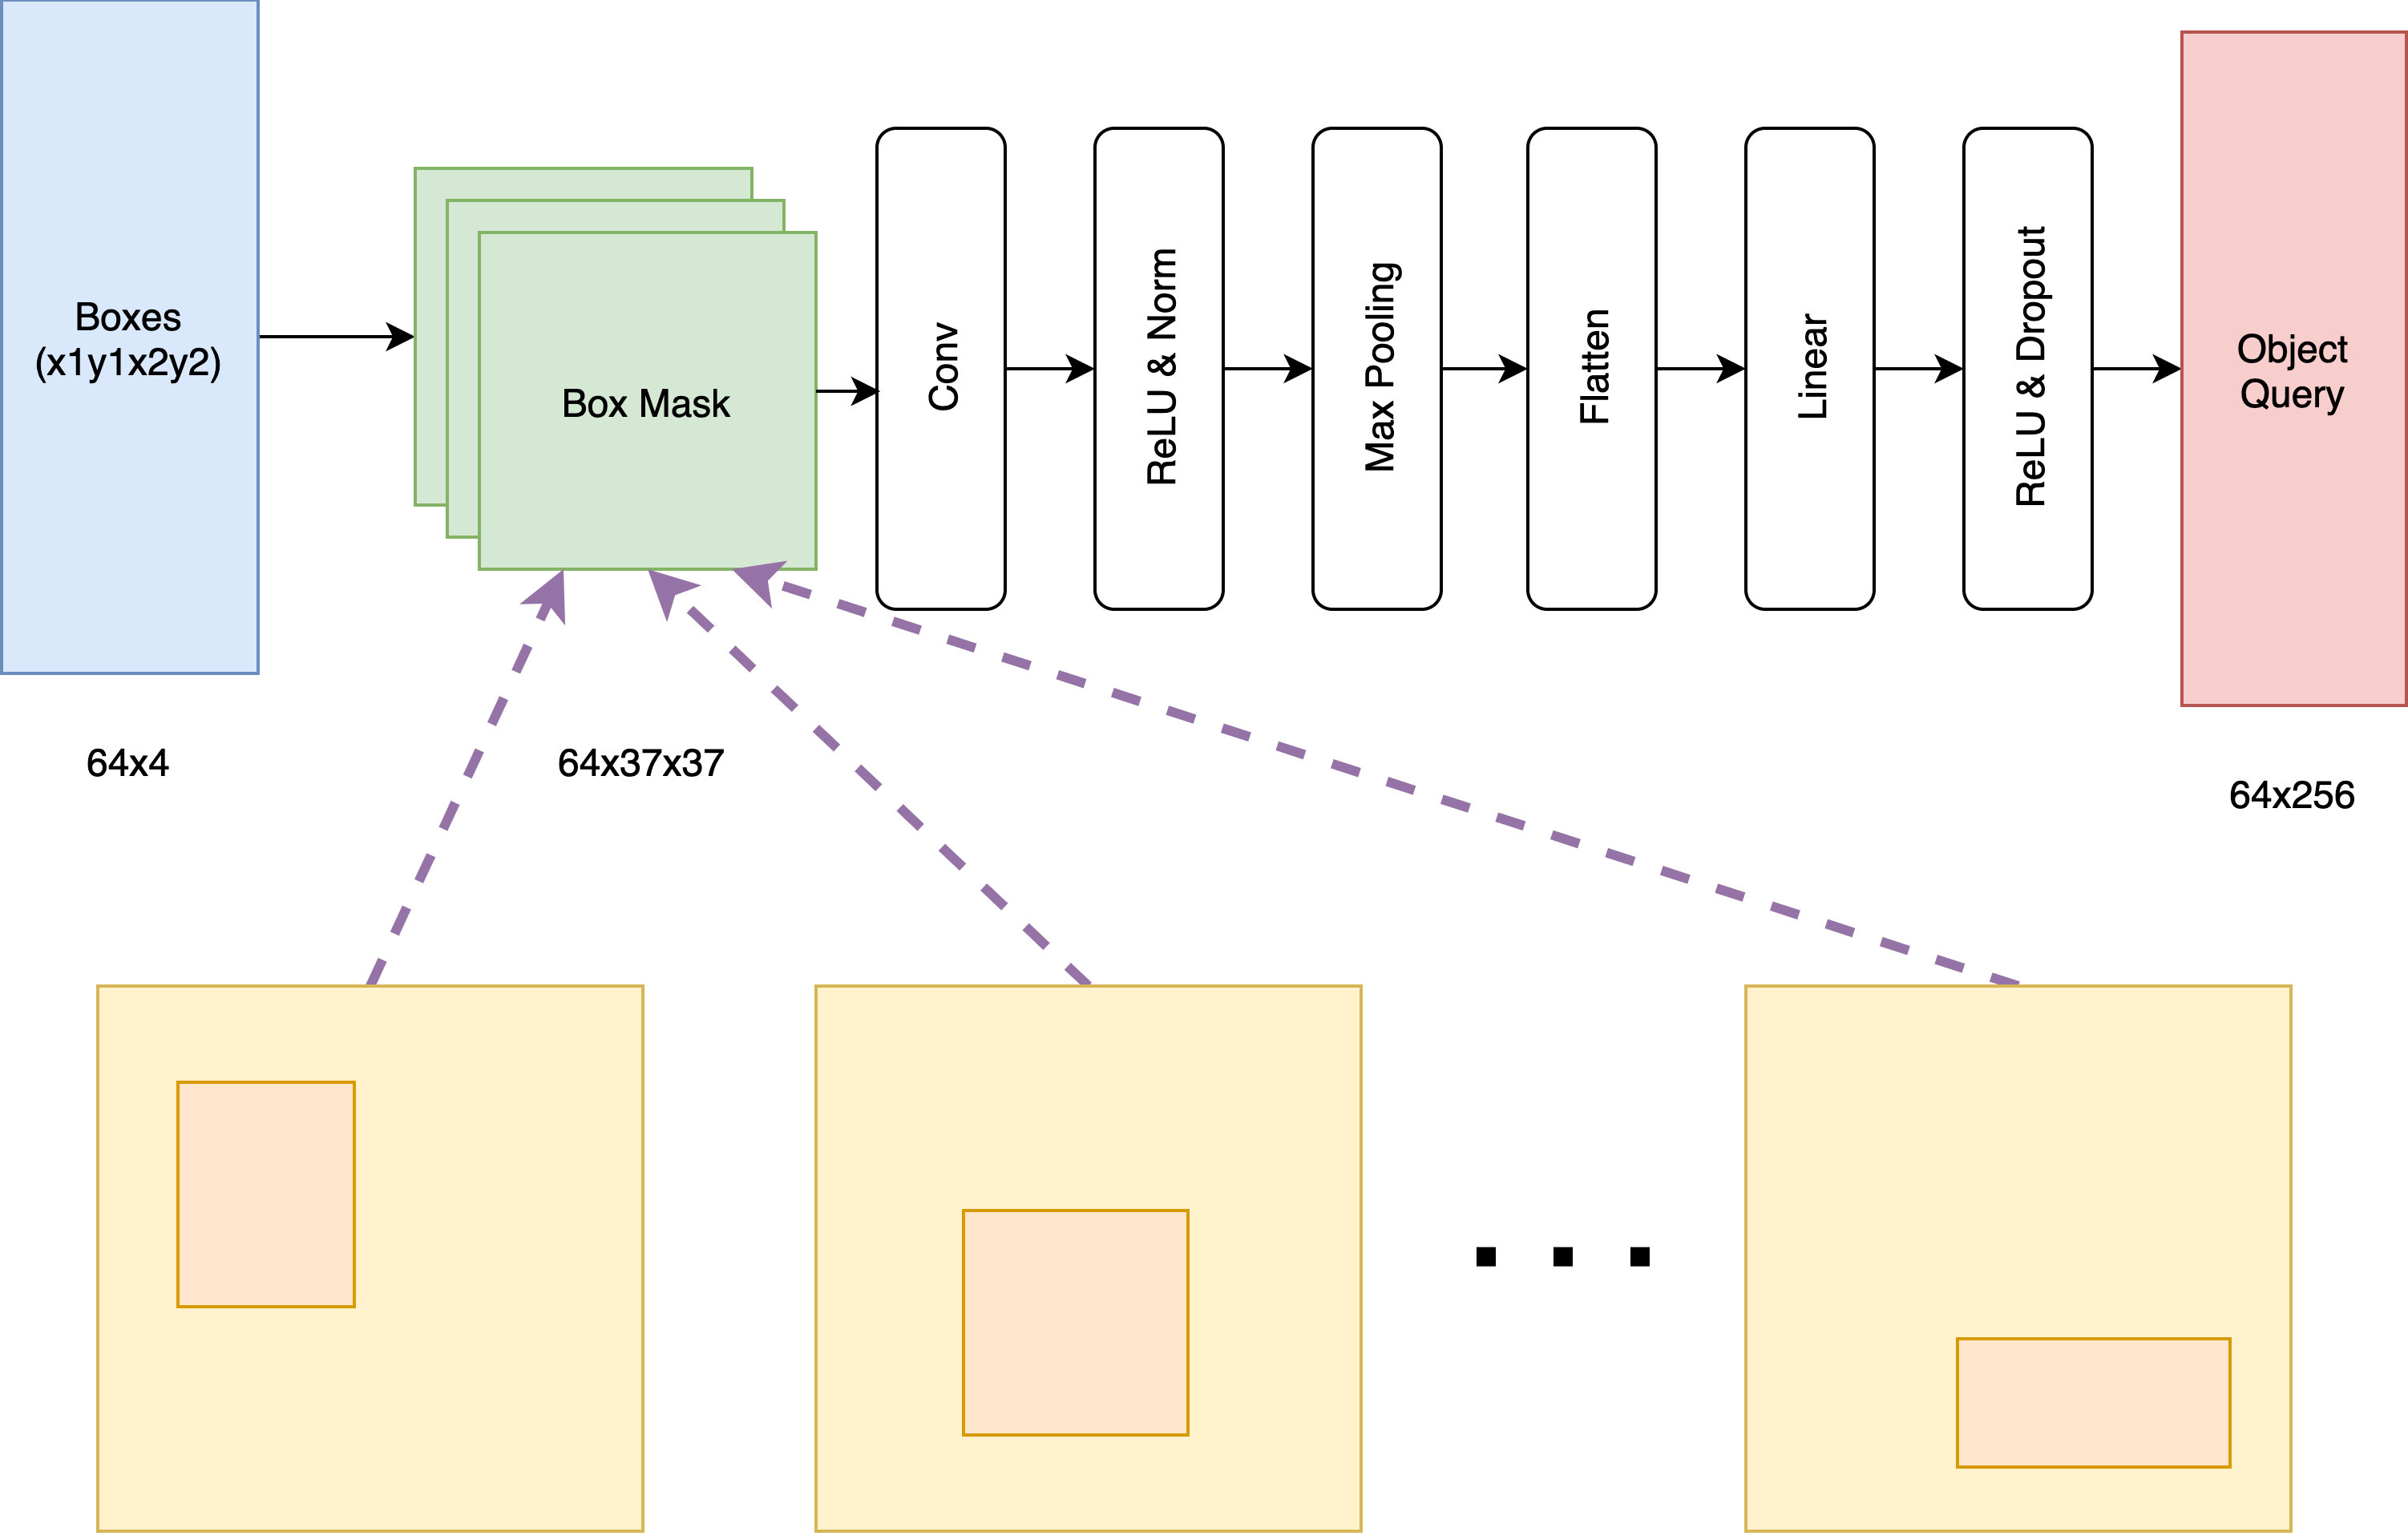
\includegraphics[width=0.8\linewidth]{figures/object_query}
	\caption[Illustration of the object query]{Illustration of the object query.}
	\label{fig:objectquery}
\end{figure}


\subsubsection{Generation of Object Feature Maps }

As shown in Figure~\ref{fig:objectquery}, we obtain the object feature through the first two Multihead Attention modules, and the process is similar to that in DETR. The difference is that we use different object queries for different tasks, as mentioned above.

For tasks PREDCLS and SGCLS, we use custom object querries. Since the query and bounding box information correspond one-to-one, the generated object features are also one-to-one correspondence, which we will prove through experiments in the next chapter.

For the task SGDET, we use a learnable query to generate the object feature, which has no corresponding relationship, and we use the Hungarian matching algorithm to find the optimal object feature with the smallest cost.

First, we obtain the predicted distributions of classes and bounding boxes through two different feed forward networks(FFN). Let us denote by $ y $ the ground truth set of objects, and $  \hat{y}= \{ \hat{y}_i\} ^N_{i=1} $ the set of $ N  $predictions.To find a bipartite matching between these two sets we search for a permutation of $ N $ elements $sigma \in \Theta _N $ with the lowest cost:
\begin{equation}\label{equ:matcher}
 \hat{\sigma} = \underset{\sigma \in \Theta _N }{argmin} \sum_{i}^{N} \mathcal L_{match} (y_i,\hat{y}_{\sigma(i)})
\end{equation}

where $\mathcal L_{match} (y_i,\hat{y}_{\sigma(i)})$ is a pair-wise matching cost between ground truth $ y_i $ and a prediction with index $ \sigma(i) $

Then we use the \textit{Hungarian loss }in DETR~\cite{carion2020end} to calculate the loss function:
\begin{equation}\label{equ:hungarianloss}
	\begin{aligned}
	&\mathcal L_{Hungarian}(y,\hat{y} ) = \sum^{N}_{i=1}[-\log{\hat{p}_{\hat{\sigma}(i)}(c_i)} + \mathbb{I}_{\{c_i \ne  \varnothing \}}\mathcal{L}_{box}(b_i,\hat{b}_{\hat{\sigma}(i)})   ], \\
	&wehre \\
	&\mathcal{L}_{box}(b_i,\hat{b}_{\hat{\sigma}(i)}) = \lambda_{iou}\mathcal{L}(b_i,\hat{b}_{\sigma(i)}) + \lambda_{L1}\left \| b_i - \hat{b}_{\sigma (i)}  \right \| _1
	\end{aligned}
\end{equation}

where $ \hat{\sigma} $ is the optimal assignment computed in the Equ.~\ref{equ:matcher}. we define probability of class $ c_i $ as $ \hat{p}_{\hat{\sigma}(i)}(c_i)$ and the predicted box as $ \hat{b}_{\sigma(i)} $. we use a linear combination of a negative log-likelihood for class prediction and a linear combination of the $  l_1  $ loss and the generalized IoU~\cite{rezatofighi2019generalized} loss for the box prediction.


\subsubsection{Object Context}

As shown in Figure~\ref{fig:objectdecoder}, we obtain the object context in the third Multihead Attention module. Its specific operation is shown in Figure~\ref{fig:objcontext}. We have given a simple example according to Equ.~\ref{equ:self_attention}. Before computing the object decoder for the first time, we initialize the object context to a tensor with 0. Assuming that we have 5 entities in the picture, before we calculate the context, the object feature size obtained from the previous calculation is $ [64, 256] $, and 59 positions will be paded by $\emptyset$. After softmax, we will Obtain a $ 64 \times 64  $ attention weight matrix (the red matrix in the figure), its meaning is the attention of each object and other objects, such as $ A_{23}$ is the attention of $ object_2 $ to $ object_3 $, and finally multiplied by the object feature we will get the object context (the yellow vector in the figure). The context of $ object_1  $is $ \sum(A_{1i}f_{obj}^i) $, that is, the context of $ object_1 $ to other $ object_i $.

\begin{figure}[tbph!]
	\centering
	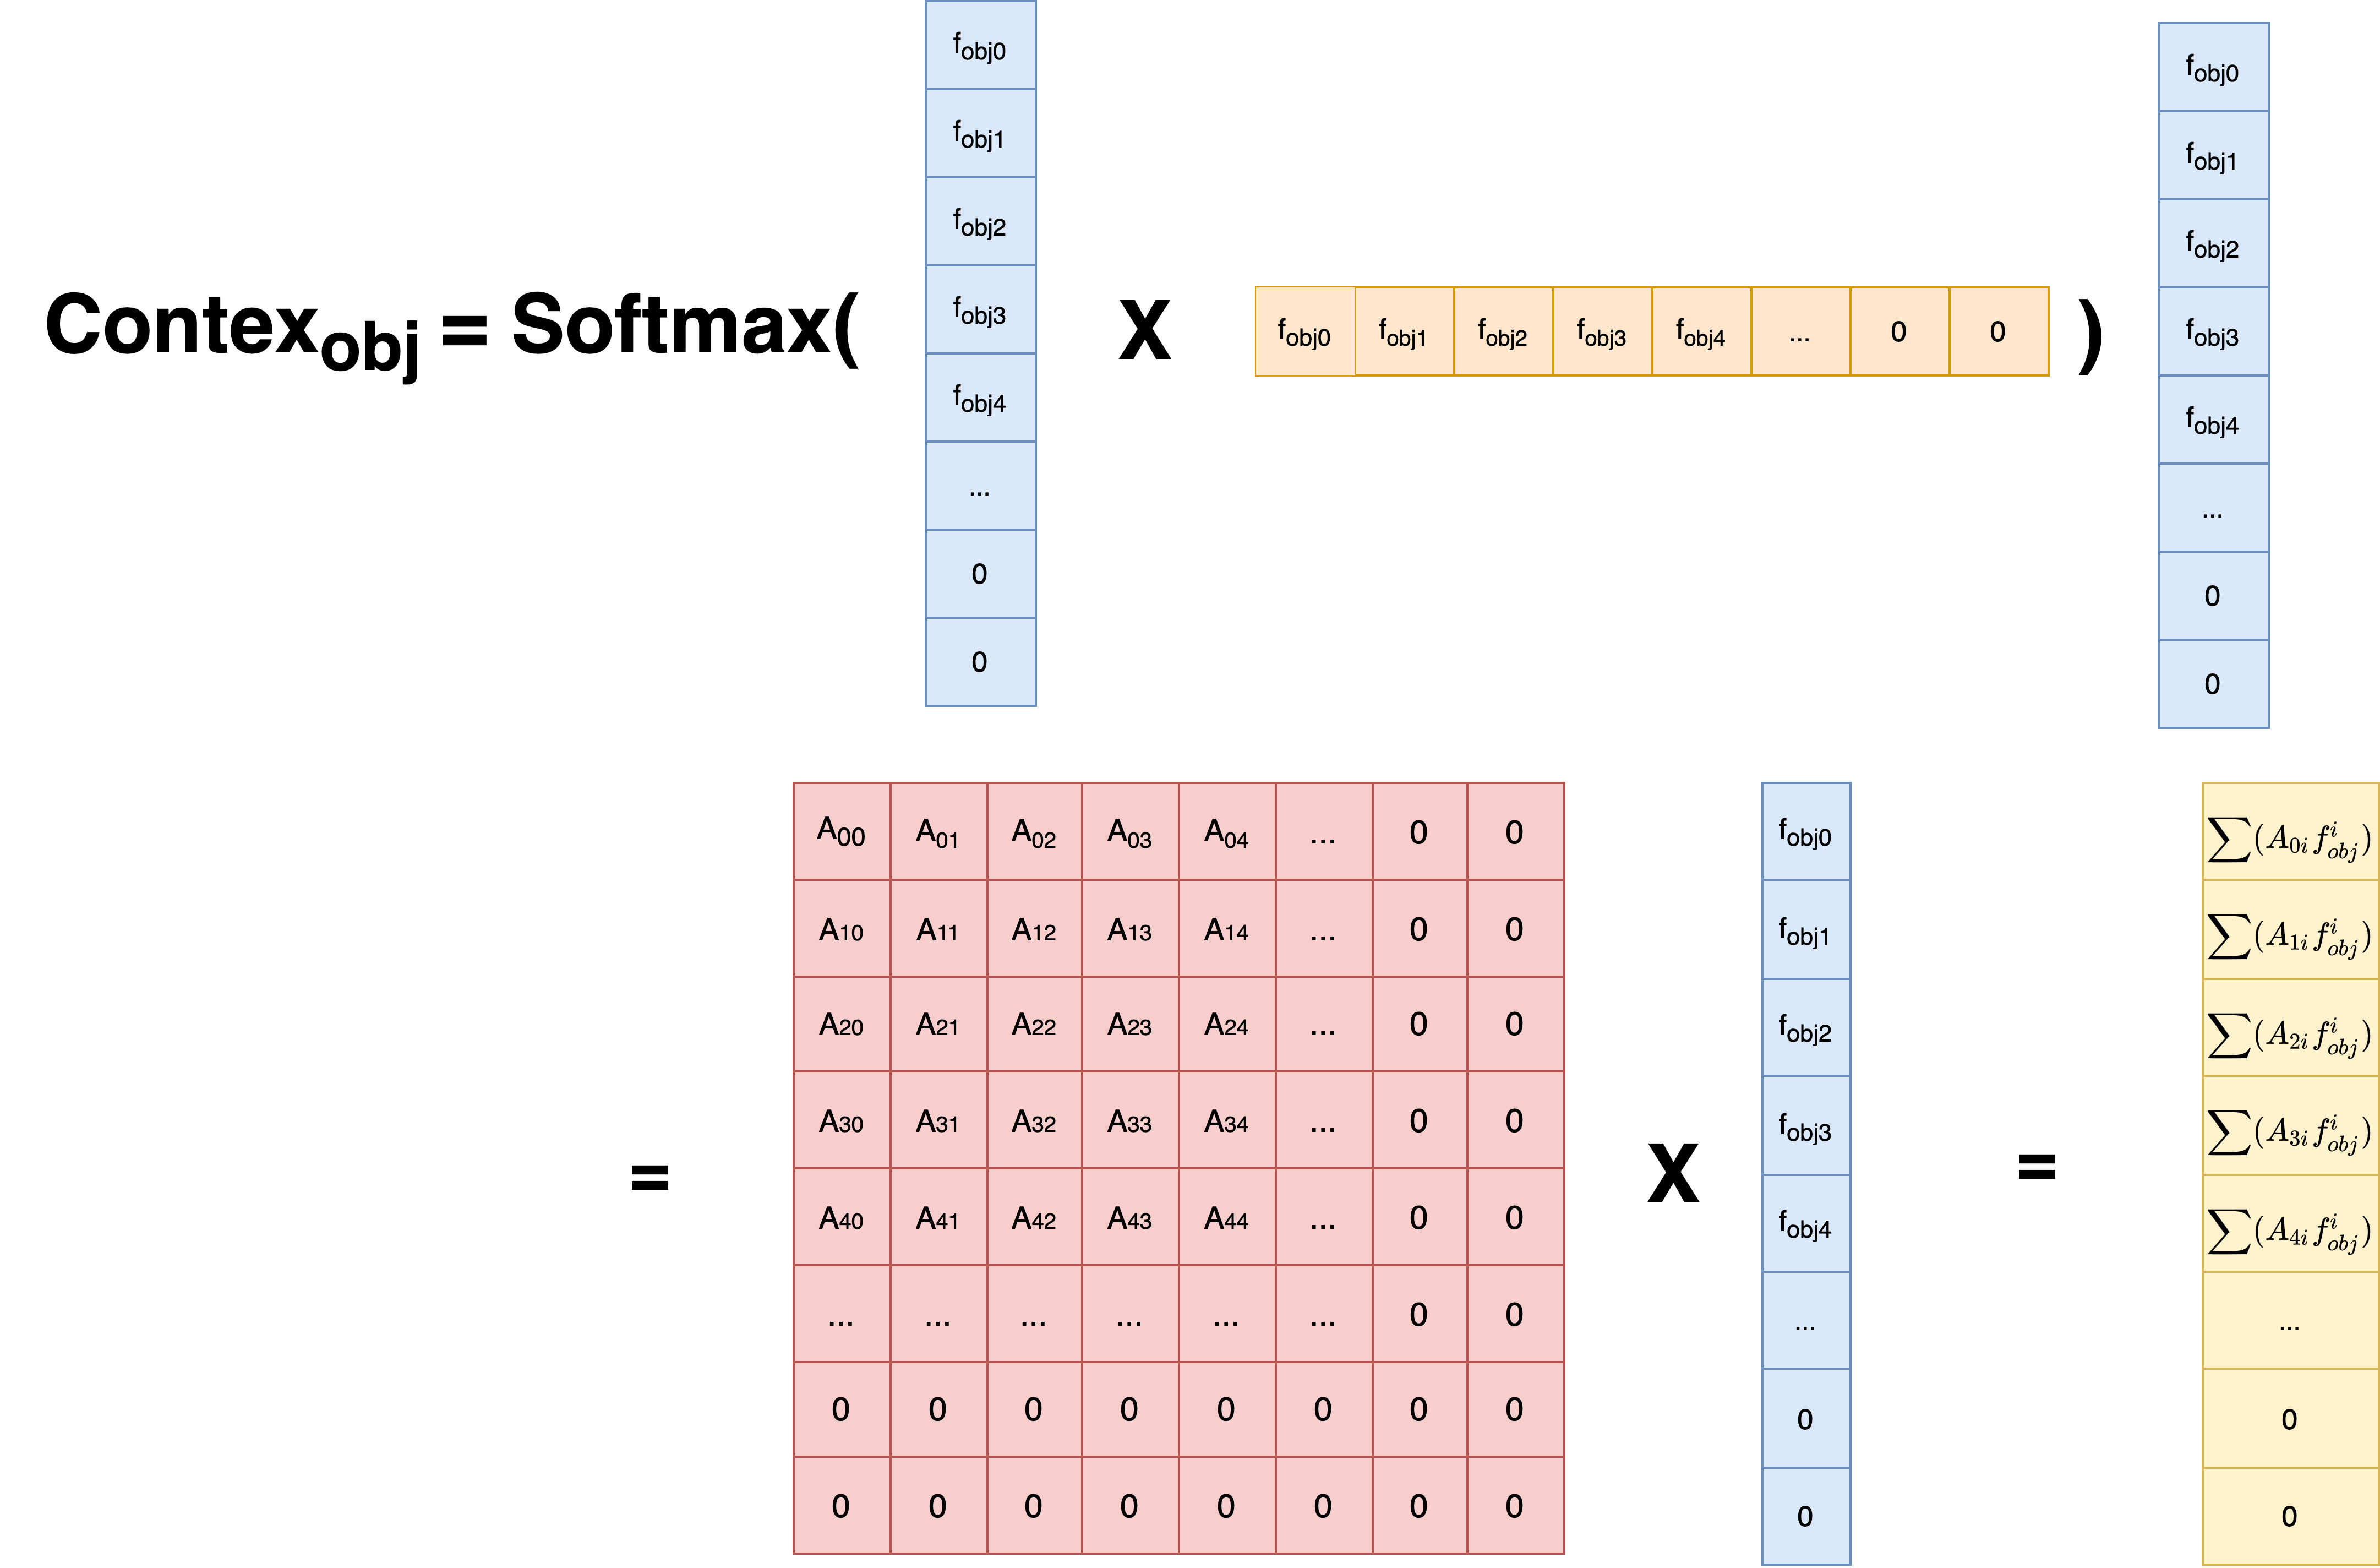
\includegraphics[width=1\linewidth]{figures/obj_context}
	\caption[A simple example of the  Object Context generation.]{A simple example of object context generation. In the first layer of decoder, we set the initial value of object context to 0. The Object Feature size is $ [64, 256] $, we assume that this picture has 5 entities, and the remaining 59 objects will be padded by 0.}
	\label{fig:objcontext}
\end{figure}


\subsection{Relation Decoder}

Our relation decoder is a typical Decoder structure consisting of two Multihead Attention modules(see in Fig.~\ref{fig:relationdecoder}). Our relationship query is customized and generated by the relationship pair $<subject,objtect>$. For example, if we have 10 entities, then we have 90 pairs, and then 90 relation queries are generated. We select the subject bounding box and object bounding box in each pair to generate two box masks, and then obtain the relation query  through the convolutional layer and the linear layer (see in Fig.~\ref{fig:relationquery}).



\begin{figure}[tbph!]
	\centering
	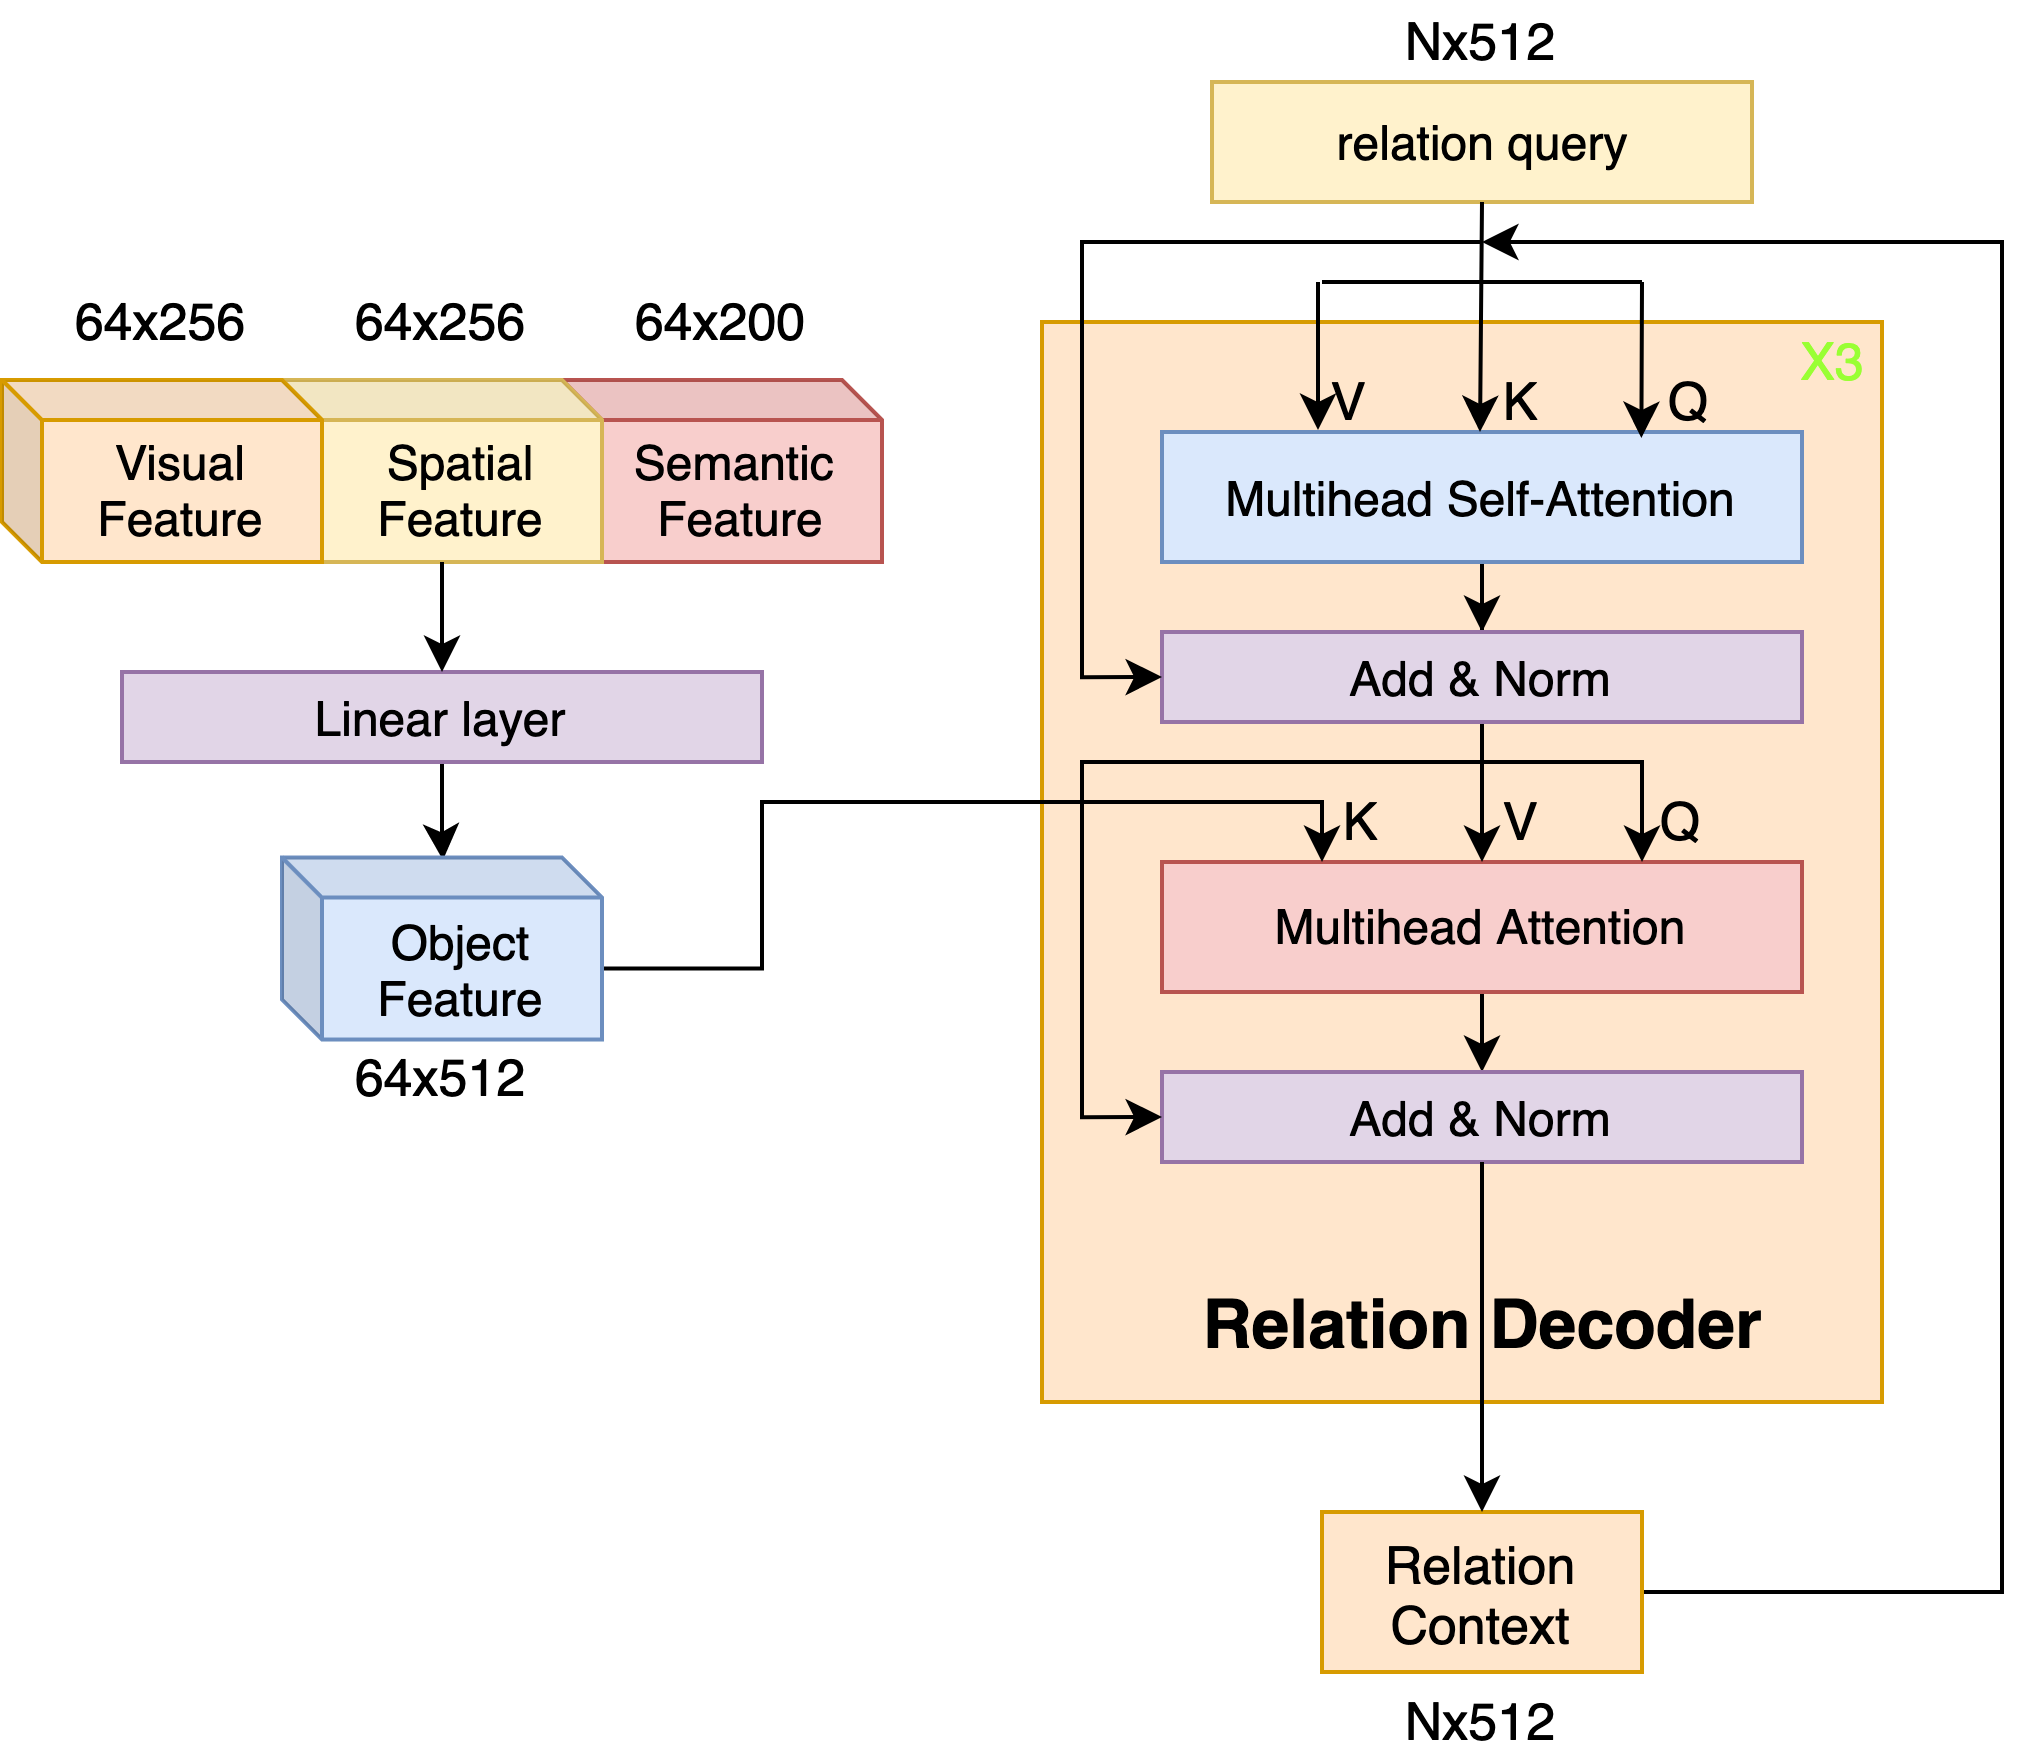
\includegraphics[width=1\linewidth]{figures/relation_decoder}
	\caption[Illustration of Relation Decoder]{Illustration of Relation Decoder.}
	\label{fig:relationdecoder}
\end{figure}

\begin{figure}[tbph!]
	\centering
	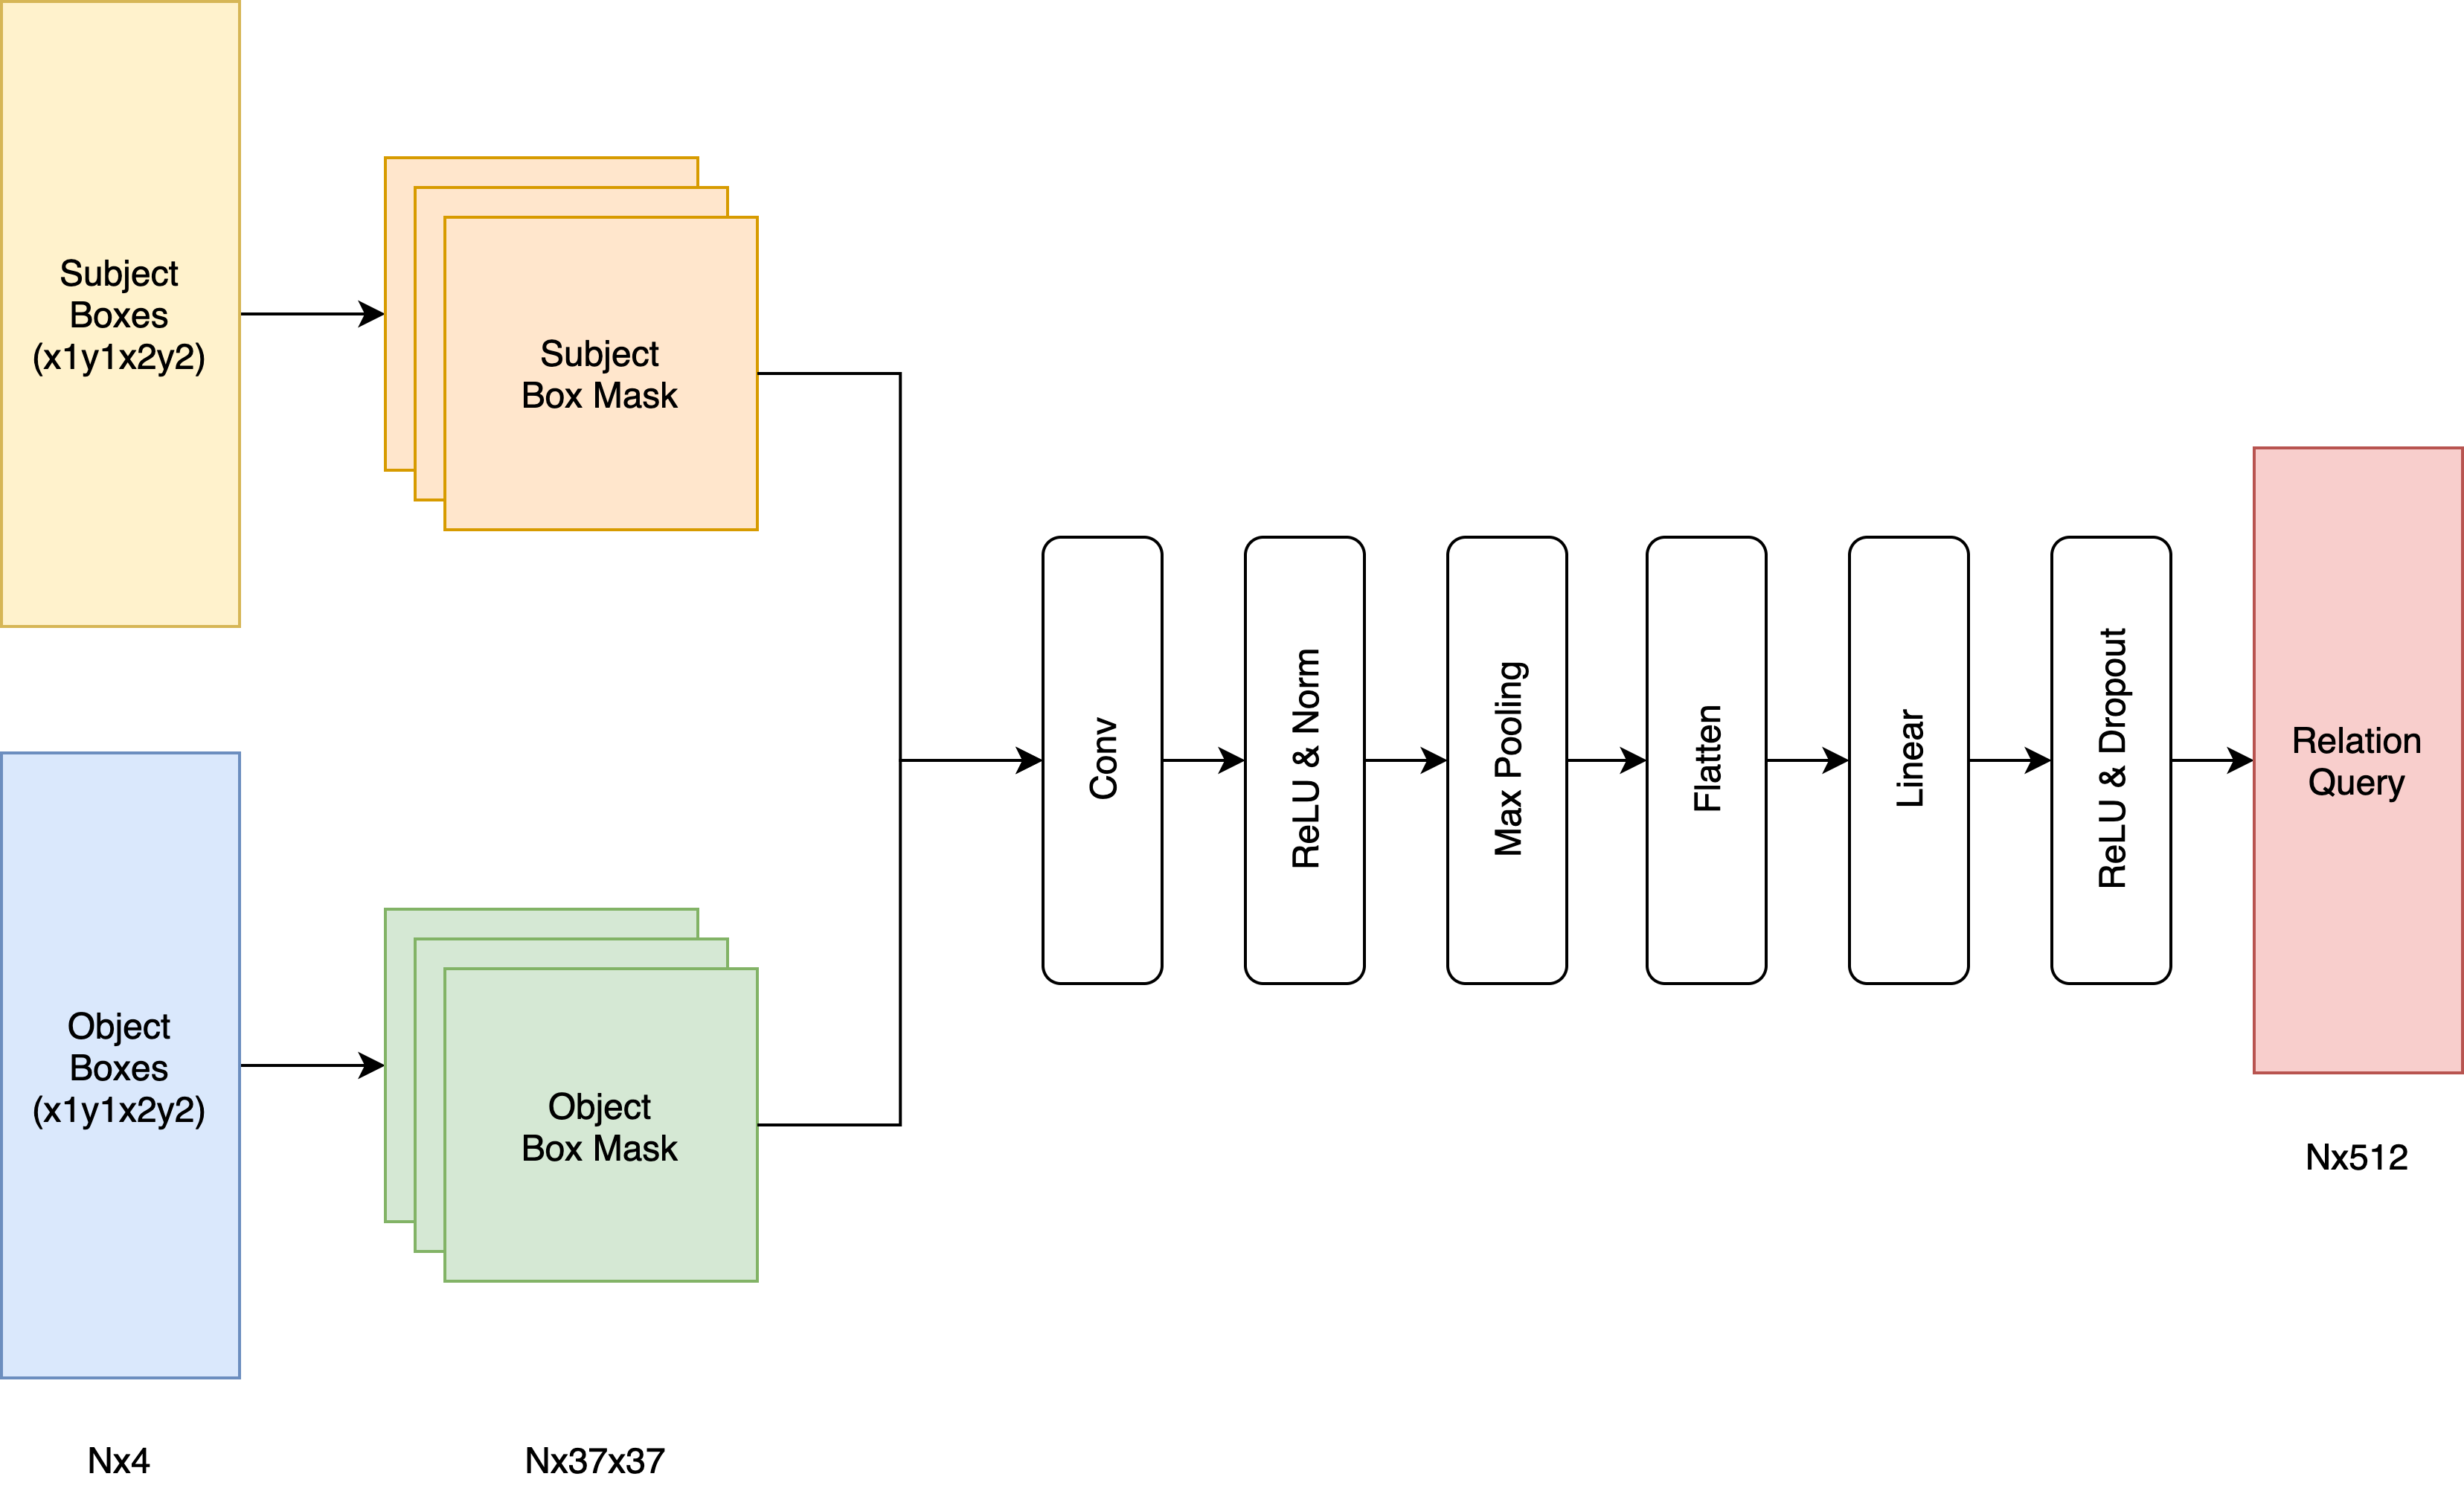
\includegraphics[width=1\linewidth]{figures/relation_query}
	\caption[Illustration of the relation query]{Illustration of the relation query. N is the number of the relation pair.}
	\label{fig:relationquery}
\end{figure}

Our relation context is the context of each relation for all objects. We use visual feat, spatial feature and  semantic feature to jointly represent object: $$f_{obj} = concat(f_{vis},f_{spt},f_{sem})$$ Among them, the visual feature $f_{vis}$ is the object feature obtained through the object decoder. The semantic feature $ f_{sem} $ is a tensor containing the semantic information of entities obtained by encoding the category through GloVe~\cite{pennington2014glove}. The spatial feature $ f_{spt} $ is a feature that contains the spatial location information of the entity. We can get it through the bounding box. In our thesis, the attention map obtained in the object decoder also has good spatial location information, so we also use the extraction of the attention map to obtain the spatial feature.



\subsection{Predicate Classifier}
Predicate prediction is a very important task in VRD problems. We get the features and context from the previous module to predict the predicate, as shown in Figure~\ref{fig:predicateclassifer}. The calculation process is shown in the following equation:

$$ score_{pred}(i,j) = Linear(concat(feat_{obj}^i, context_{rel}^{ij}, context_{obj}^i, feat_{obj}^j) $$

where $ i $ is the index of subject, $ j $ is the index of object,  $ feat_{obj} $ is the visual feature obtained from the Object Decoder, so $ feat_{obj}^i $ is the visual feature of the subject, and the $ feat_{obj}^j $ is the visual feature of the object. $ context_{rel}^{ij} $ is the relation context of the realtion $ pair(subject_i,object_j)  $obtained from the Relation Decoder, $  context_{obj}^i $ is the object context of the $subject_i$ obtained from the Object Decoder.

 \begin{figure}[tbph!]
 	\centering
 	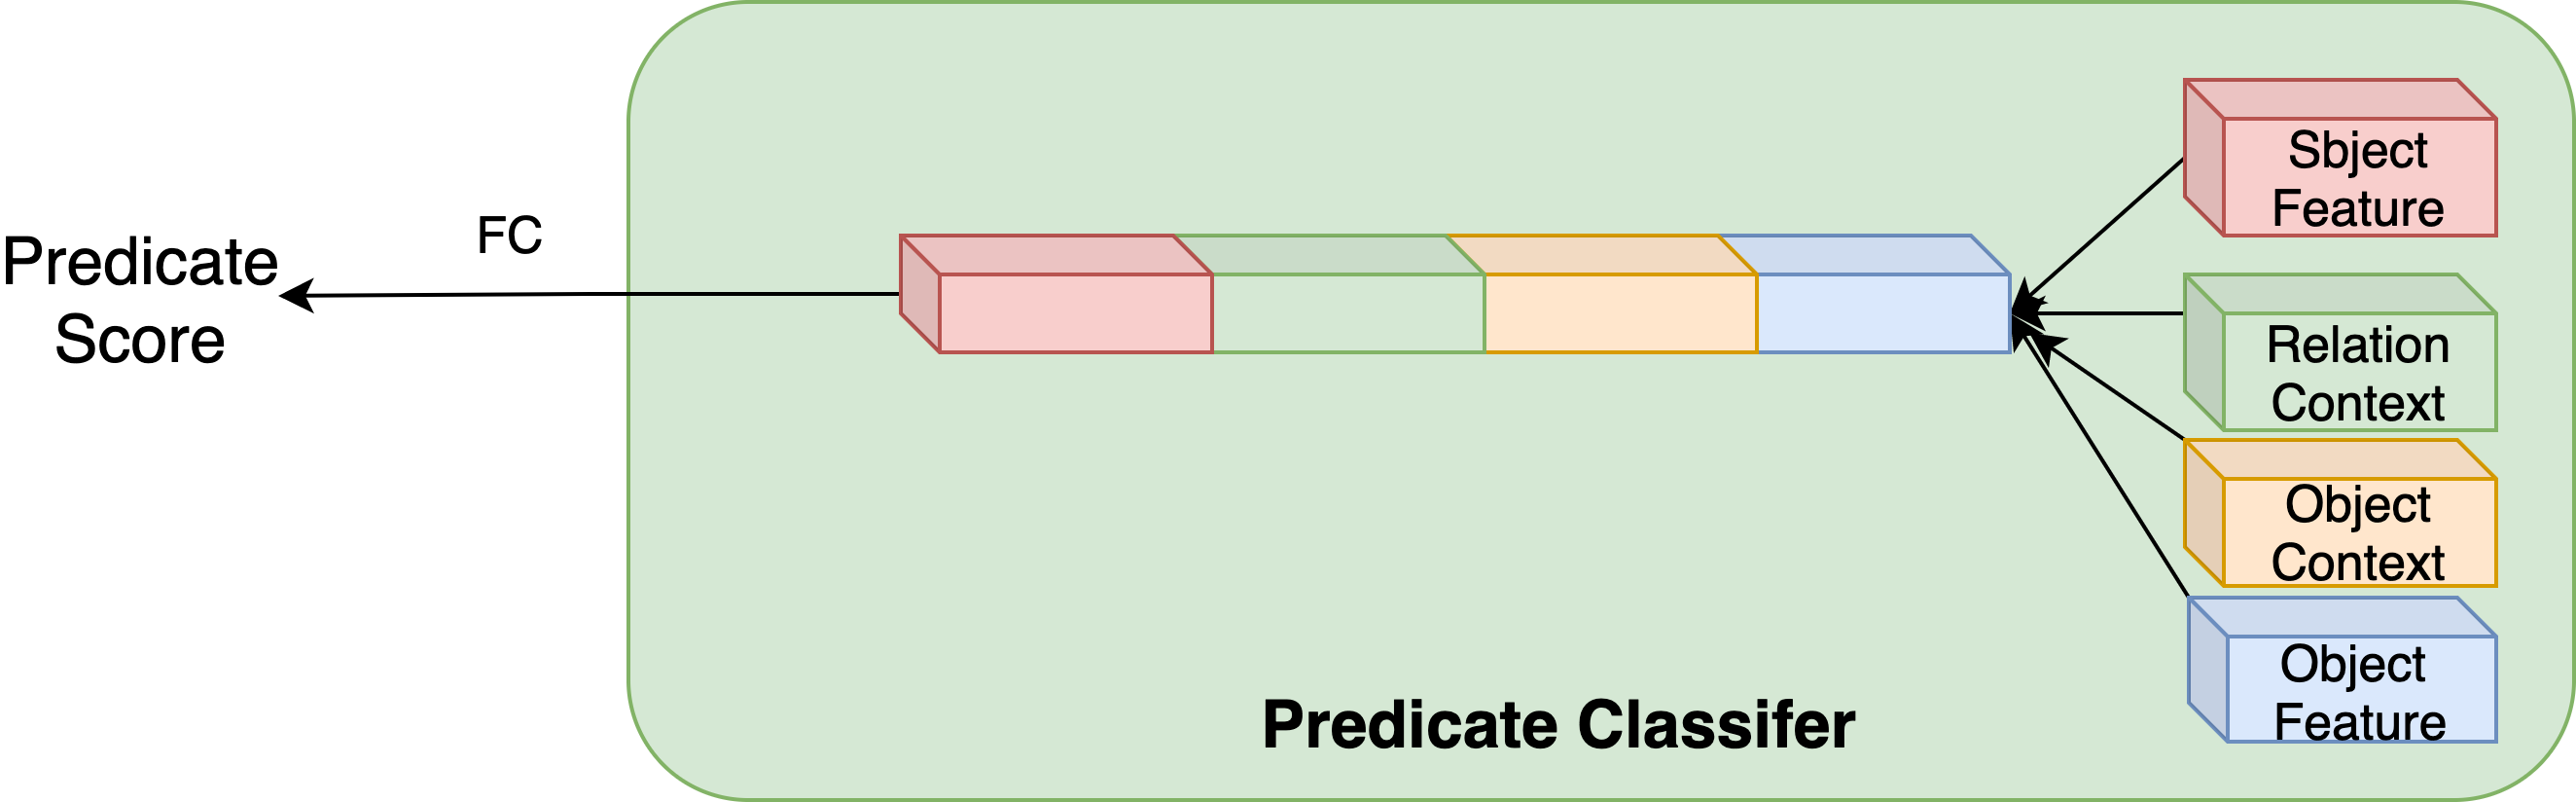
\includegraphics[width=1\linewidth]{figures/predicate_classifer}
 	\caption[Illustration of the predicate classfier]{Illustration of the predicate classfier.}
 	\label{fig:predicateclassifer}
 \end{figure}
 
 
 \begin{figure}[h]
 	\centering
 	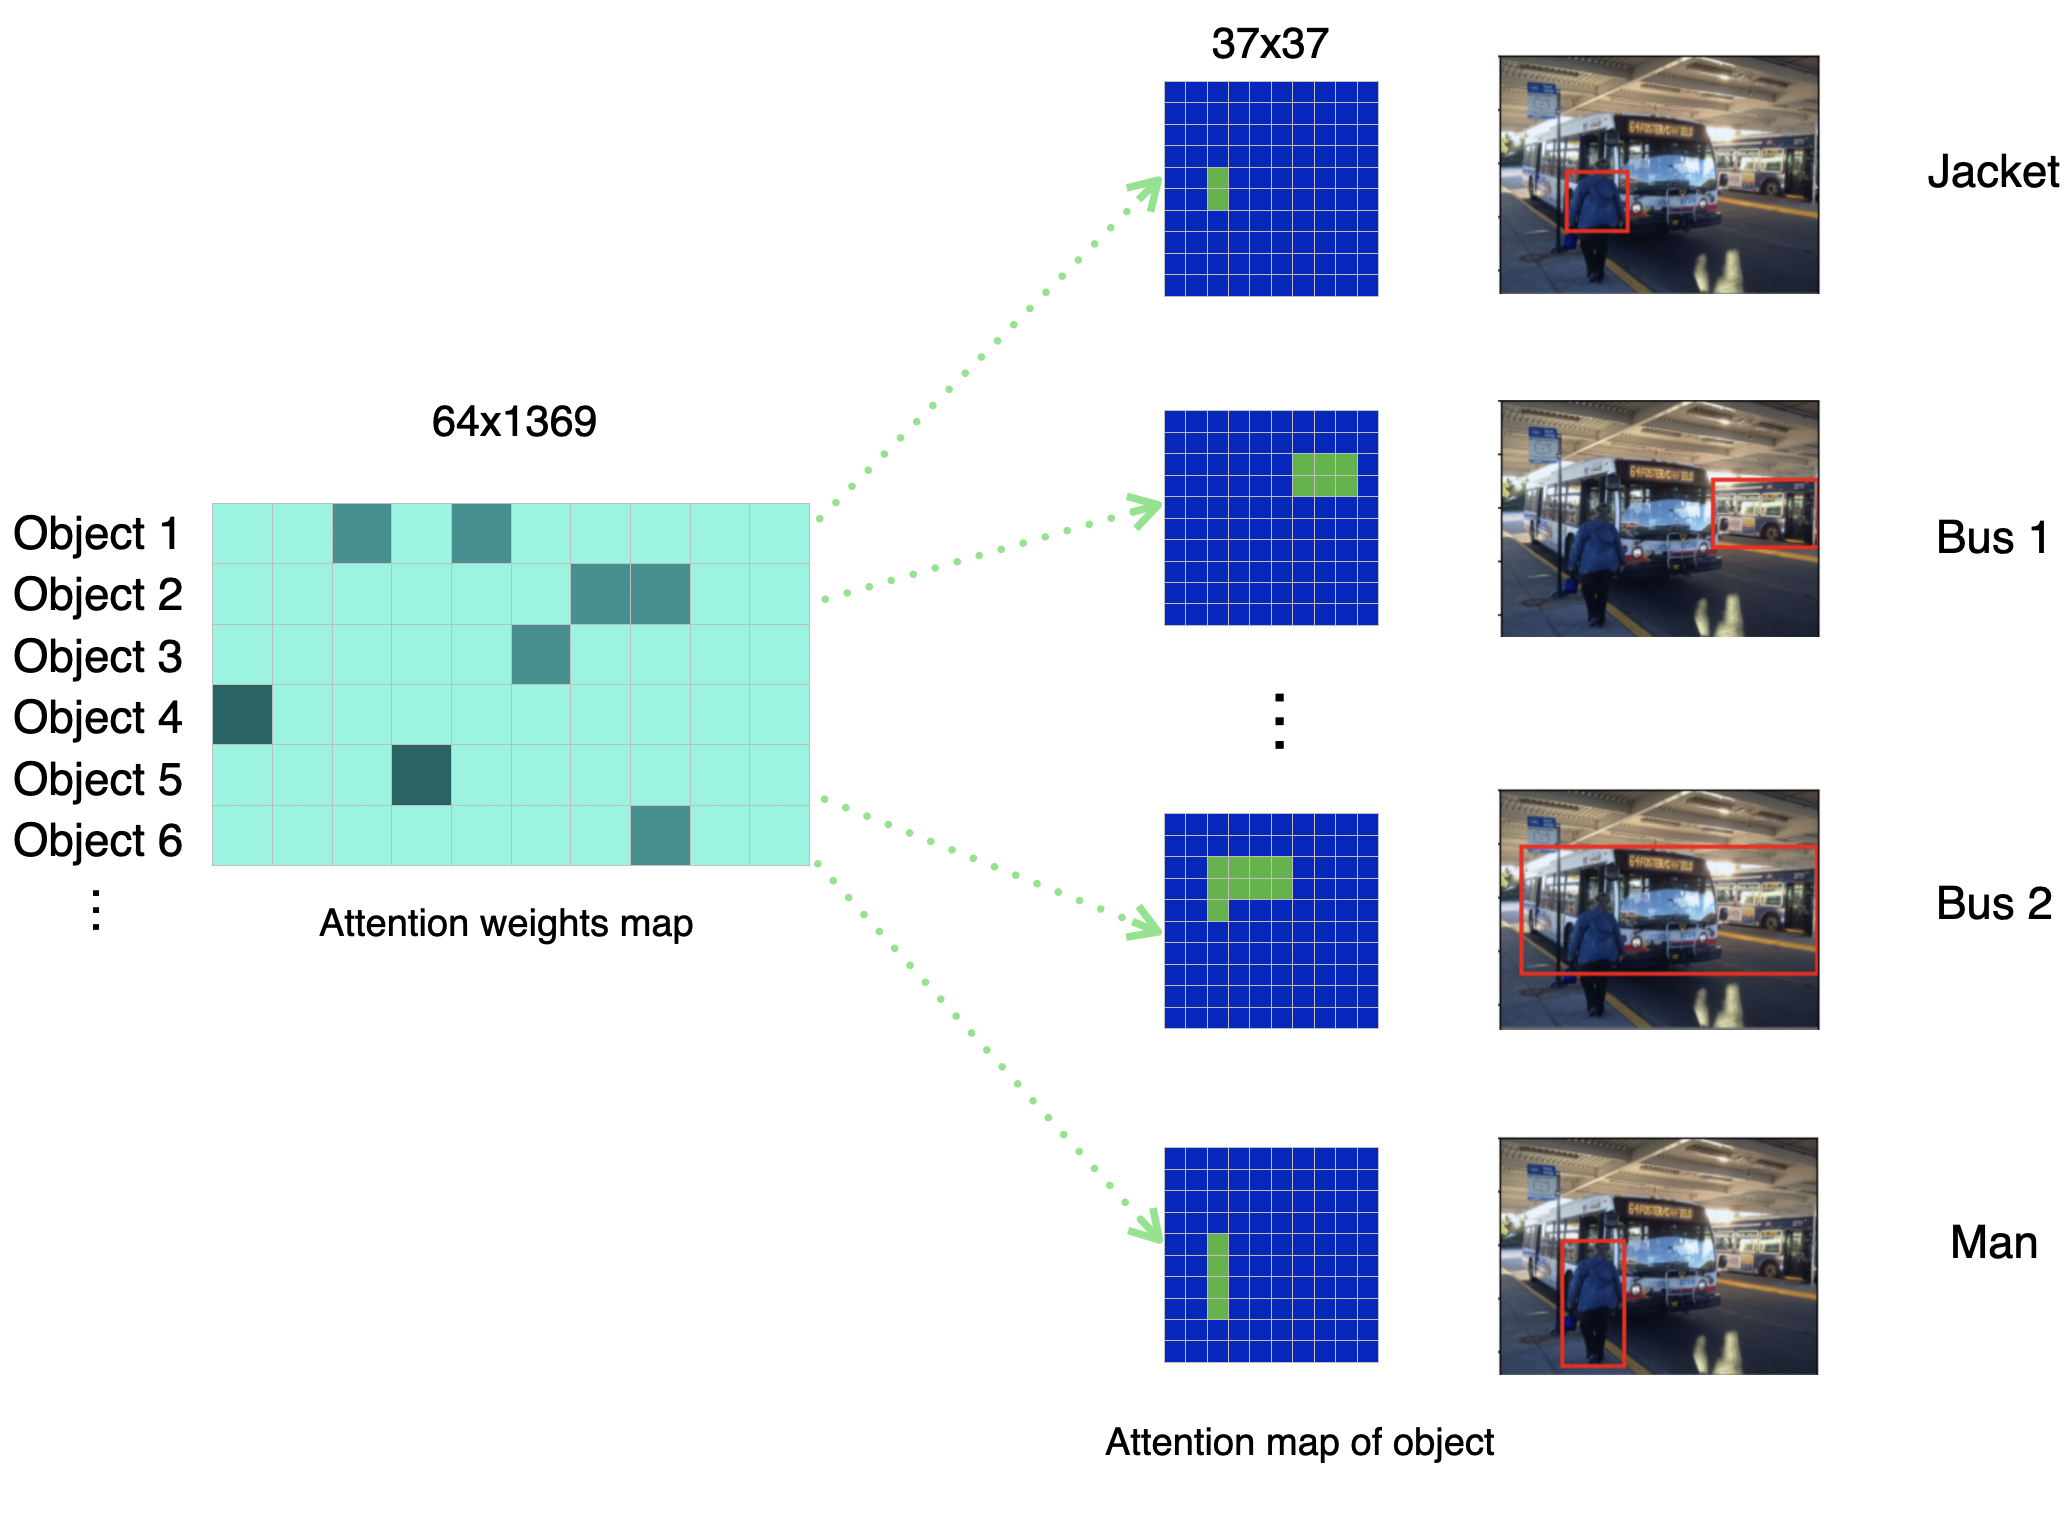
\includegraphics[width=0.8\linewidth]{figures/attention_map}
 	\caption[Illustration of the attention map]{Each row in the attention weights map represents the attention of each object. }
 	\label{fig:attentionmap}
 \end{figure}
 

\subsection{Attention Loss}

In the object decoder(see in Fig.~\ref{fig:objectdecoder}), we obtain the object visual feature through the second Multihead Attention module, and the attention maps size of $ [64, 1369] $. We can convert it to a tensor of $ [64, 37, 37], $ which means the attention weights of each object to each pixel in the image feature from the encoder.



As shown in Fig.~\ref{fig:attentionmap}, we get an attention weights map of size 64x1369, and each row of it can be transformed into a small attention map of 37x37 size. We hope that this attention map can have a spatial correspondence with the entity in the picture. For example, in this picture we can see a man wearing a purple jacket and two buses. We hope to find the corresponding object in the small attention map, we will find green in the attention map of the jacket. The attention weight of the part is much higher than the blue one. This shows that we pay more attention to this green area when generating the object feature of the jacket. In this way, we can better visualize the object and make our object feature better.

Therefore, we designed an attention loss according to the ranking loss, so that the attention weights of the green area are higher than that of the blue area:

\begin{equation}
	loss_{attention}=max(0, \frac{1}{m}\sum_{m}Att_j^{no\_obj}-\frac{1}{n}\sum_{n}Att_i^{obj}+0.25
	/1369)
\end{equation}

where $Att_j^{no\_obj}$ is the attention value $  j  $ of the the area outside the bounding box  of  object, $ m $ is the total number of attention values. $ Att_i^{obj} $ is the attention value $  i  $ of the the area within the bounding box  of object, $ n $ is the total number of attention values. Then $ Margin=0.25/1369  $ is quarter the average of the attention map.

